\documentclass[11pt,a4paper]{article}
\usepackage[T1]{fontenc}\usepackage[utf8]{inputenc}\usepackage{lmodern}
\usepackage[margin=25mm]{geometry}
\usepackage{amsmath,amssymb,graphicx,booktabs,array,microtype,float,placeins,caption}
\usepackage[hidelinks]{hyperref}\usepackage{fancyhdr}
\setlength{\headheight}{14pt}\pagestyle{fancy}\fancyhf{}
\fancyhead[L]{Centrifugal Pump Impeller Design}\fancyhead[R]{Project One}\fancyfoot[C]{\thepage}
\setlength{\parindent}{0pt}\setlength{\parskip}{6pt}
\captionsetup{font=small,labelfont=bf}
\hypersetup{pdftitle={Centrifugal Pump Impeller Design},pdfauthor={Pouya Asghari and Niloufar Fattahi}}
\begin{document}
\begin{titlepage}\centering

\includegraphics[height=23mm]{figures/rId8.png}\hfill
\includegraphics[height=23mm]{figures/rId9.png}\par
\vspace{18mm}{\Large Turbomachinery\par}\vspace{10mm}
{\huge\bfseries Centrifugal Pump Impeller Design\par}\vspace{5mm}
{\Large Analytical Construction and CFturbo Modeling\par}\vspace{5mm}
{\large Project One Report\par}\vspace{18mm}
{\Large Pouya Asghari\par}\vspace{4mm}{\Large Niloufar Fattahi\par}\vspace{10mm}
Instructor: Dr. Riasi\par
\vfill
Second semester of academic year 1404--1405 (Iranian calendar)\par
School of Mechanical Engineering\par
College of Engineering, University of Tehran\par
\vspace{8mm}English translation of the original Persian report
\end{titlepage}
\section*{About this edition}
This is an English translation of the supplied Persian project report. The two-phase structure, equations, numerical results, CAD construction sequence, and original substantive figures are retained. Screenshot interface labels and catalog extracts remain as originally supplied. Student identification numbers are omitted, and the coauthorship shown in the source is preserved. The spelling ``Niloufar Fattahi'' is a transliteration of the Persian author name.

The source uses ``simulation'' broadly for the CFturbo workflow. The archive documents analytical design, geometry generation, and preliminary software estimates; it does not include a separate CFD mesh, solver case, residual history, or validated flow-field results. Numerical and design claims in the translated body remain the original authors' statements. An editorial appendix identifies discrepancies and compares the preliminary dimensions with parameters stored in the supplied native CFturbo file. It does not silently replace the original results.

\begingroup\small\setlength{\parskip}{0pt}\tableofcontents\endgroup\clearpage


\section{Introduction}

This project aims to develop the geometry, detailed drawings, and three-dimensional model of a centrifugal pump impeller for the 200-100 model, using the operating parameters and technical data in the Pumpiran catalog. The report is organized into two phases. In the first phase, the impeller blade geometry is designed step by step using the single-arc and double-arc methods, based on turbomachinery theory and the extracted pump duty point, and the final profile is drawn. In the second phase, the geometry and operating conditions at the catalog best efficiency point (BEP) are used for specialized pump modeling and simulation in CFturbo to examine flow behavior and design parameters.

\section{Phase One Analytical Design and Blade Construction}

\subsection{Reference duty point and initial assumptions}

The iso-efficiency curves in the Pumpiran catalog are examined at a rotational speed of $N=1450$ rpm and an impeller diameter of $D_2=209$ mm. The corrected operating coordinates below are adopted as the best efficiency point, with a maximum efficiency of 84.5\%.

Volumetric flow rate: $Q=125\ \mathrm{m^3/h}$, equivalent to approximately $0.0347\ \mathrm{m^3/s}$.

Effective head: $H=13.5$ m.

Shaft diameter at the coupling: $d_s=32$ mm. Allowing for hub thickness, the hub diameter is assumed to be $d_h=45$ mm.

\begin{figure}[H]\centering

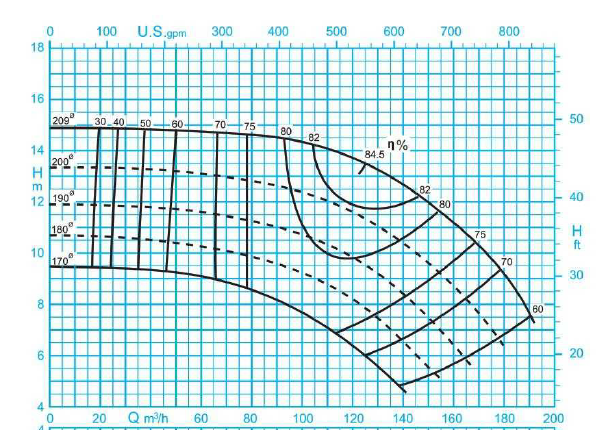
\includegraphics[width=0.94\linewidth,height=0.33\textheight,keepaspectratio]{figures/rId10.png}

\caption{Pumpiran catalog performance curves used to select the reference duty point.}\end{figure}

\subsubsection{Design assumptions}

Hydraulic efficiency: $\eta_h=0.90$.

Volumetric efficiency: $\eta_v=0.96$, allowing for 4\% internal leakage.

Blade blockage factors: $\tau_1=0.85$ at the inlet and $\tau_2=0.92$ at the outlet.

Number of blades: $Z=6$, adopted as a common choice for centrifugal water pumps.

Working fluid: water, with density $\rho=1000\ \mathrm{kg/m^3}$.

\subsection{Velocities and principal impeller dimensions}

\subsubsection{Step One Specific speed and theoretical head}

The specific speed $N_s$ is used to characterize the overall impeller form:

\[N_s=\frac{N\sqrt{Q}}{H^{0.75}}=\frac{1450\sqrt{0.0347}}{13.5^{0.75}}\approx38.3.\]

The source interprets this value as confirming a fully radial centrifugal pump. Applying the hydraulic efficiency gives the theoretical head:

\[H_{\mathrm{th}}=\frac{H}{\eta_h}=\frac{13.5}{0.90}=15.0\ \mathrm{m}.\]

\subsubsection{Step Two Outlet velocity triangle and outlet angle}

The peripheral speed at the outlet diameter $D_2=209$ mm is

\[U_2=\frac{\pi D_2N}{60}=\frac{\pi(0.209)(1450)}{60}=15.87\ \mathrm{m/s}.\]

The tangential component of the fluid velocity, $C_{u2}$, follows from Euler's equation:

\[H_{\mathrm{th}}=\frac{U_2C_{u2}}{g}\quad\Longrightarrow\quad C_{u2}=\frac{15.0(9.81)}{15.87}=9.27\ \mathrm{m/s}.\]

Assuming a blade outlet angle of $\beta'_2=35^\circ$, the Stodola slip factor is calculated as

\[\sigma=1-\frac{\pi\sin35^\circ}{Z}=1-\frac{\pi(0.573)}{6}=0.70.\]

The ideal tangential velocity is $C_{u2,\infty}=9.27/0.70=13.24\ \mathrm{m/s}$. From the outlet velocity triangle, the outlet meridional velocity is

\[C_{m2}=(U_2-C_{u2,\infty})\tan\beta'_2=(15.87-13.24)\tan35^\circ=1.84\ \mathrm{m/s}.\]

The corrected flow rate is $Q'=Q/\eta_v=0.0361\ \mathrm{m^3/s}$. The outlet blade width is therefore

\[b_2=\frac{Q'}{\pi D_2 C_{m2}\tau_2}=\frac{0.0361}{\pi(0.209)(1.84)(0.92)}=0.032\ \mathrm{m}=32\ \mathrm{mm}.\]

\subsubsection{Step Three Inlet dimensions and inlet angle}

Taking the suction flange diameter of 125 mm as the reference, the impeller eye diameter is chosen as $D_1=125$ mm. The effective inlet area is

\[A_1=\frac{\pi}{4}(D_1^2-d_h^2)=\frac{\pi}{4}(0.125^2-0.045^2)=0.0107\ \mathrm{m^2}.\]

The inlet meridional velocity is

\[C_{m1}=\frac{Q'}{A_1}=\frac{0.0361}{0.0107}=3.37\ \mathrm{m/s}.\]

The inlet peripheral speed is

\[U_1=\frac{\pi D_1N}{60}=\frac{\pi(0.125)(1450)}{60}=9.49\ \mathrm{m/s}.\]

Assuming zero inlet prewhirl, $C_{u1}=0$, the inlet relative-flow angle is

\[\beta_{f1}=\arctan\left(\frac{C_{m1}}{U_1}\right)=\arctan\left(\frac{3.37}{9.49}\right)\approx19.5^\circ.\]

Allowing for a suitable incidence angle, the inlet blade metal angle is set to $\beta'_1=25^\circ$.

The inlet blade width is

\[b_1=\frac{Q'}{\pi D_1 C_{m1}\tau_1}=\frac{0.0361}{\pi(0.125)(3.37)(0.85)}=0.032\ \mathrm{m}=32\ \mathrm{mm}.\]

\subsection{Blade geometry using single and double arcs}

For the SolidWorks construction, the inlet radius is $R_1=62.5$ mm and the outlet radius is $R_2=104.5$ mm. Blade angles are measured from the tangents to the corresponding circles.

\subsubsection{Single arc method}

In this method, the entire blade profile is represented by one circular arc of constant radius $R_{\mathrm{arc}}$:

\[R_{\mathrm{arc}}=\frac{R_2^2-R_1^2}{2(R_2\cos\beta'_2-R_1\cos\beta'_1)}.\]

\[R_{\mathrm{arc}}=\frac{104.5^2-62.5^2}{2(104.5\cos35^\circ-62.5\cos25^\circ)}\approx120.9\ \mathrm{mm}.\]

The source specifies a single-arc blade radius of 120.9 mm, with the arc center located at a radial distance of 69.6 mm from the shaft center.

\paragraph{Construction procedure}

First, draw two concentric circles with radii $R_1$ and $R_2$ in SolidWorks.

\begin{figure}[H]\centering

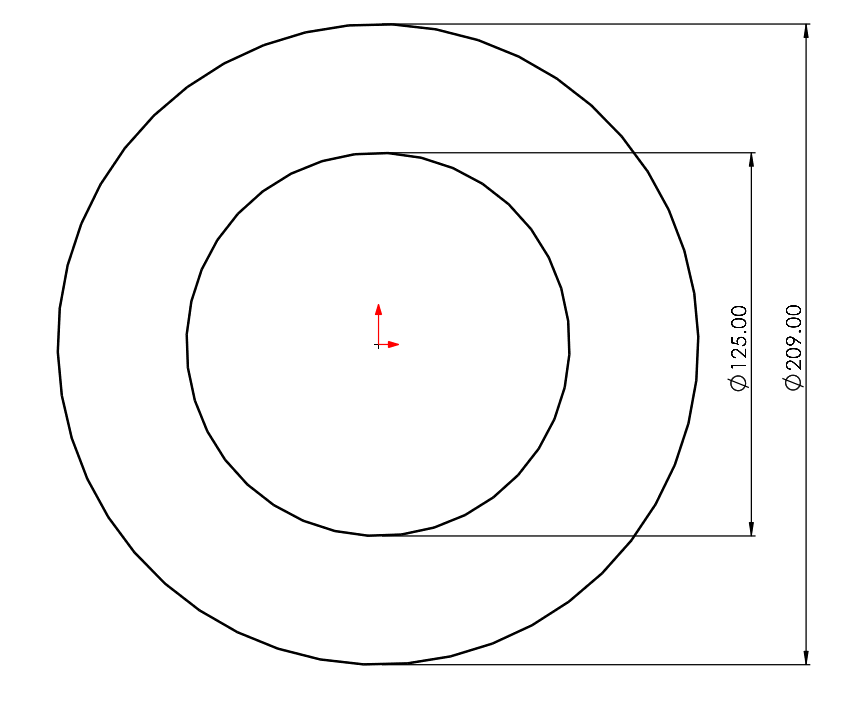
\includegraphics[width=0.94\linewidth,height=0.33\textheight,keepaspectratio]{figures/rId11.png}

\caption{Concentric inlet and outlet circles for the single arc construction.}\end{figure}

Choose an arbitrary point $B$ on the outer circle and join it to the common center $O$. Select a point $K$ on the inner circle so that $\angle BOK=\beta'_1+\beta'_2$:

\[\beta'_1+\beta'_2=25^\circ+35^\circ=60^\circ.\]

\begin{figure}[H]\centering

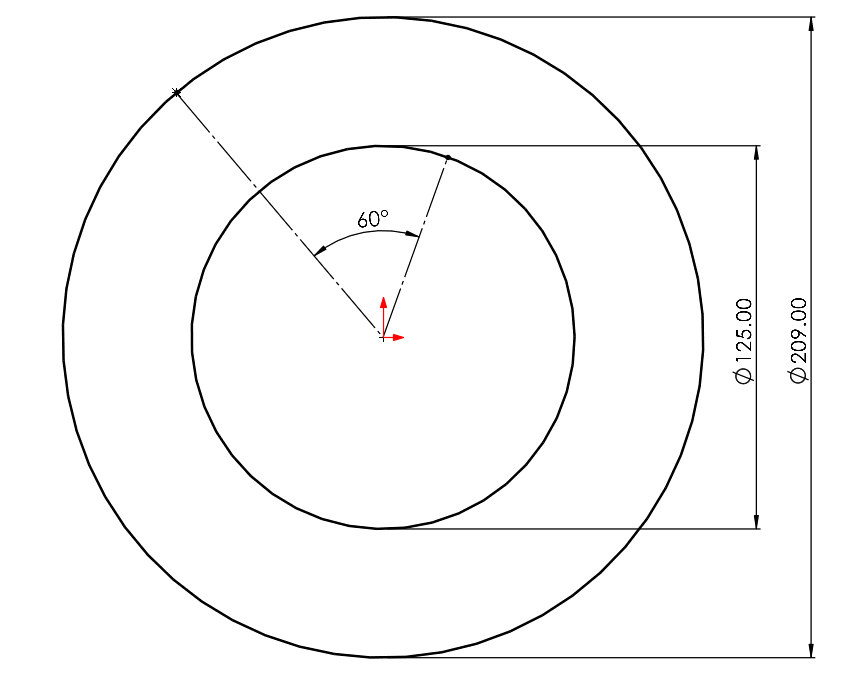
\includegraphics[width=0.94\linewidth,height=0.33\textheight,keepaspectratio]{figures/rId13.png}

\caption{Selection of points B, O, and K with a central angle of 60 degrees.}\end{figure}

Join $B$ to $K$ and extend the line until it intersects the inner circle again; call this intersection $A$. Draw the perpendicular bisector of $BA$. From $B$, draw a line at an angle $\beta'_2$ to $BO$ so that it intersects the perpendicular bisector at $G$. Finally, draw an arc from $B$ to $A$ centered at $G$.

\begin{figure}[H]\centering

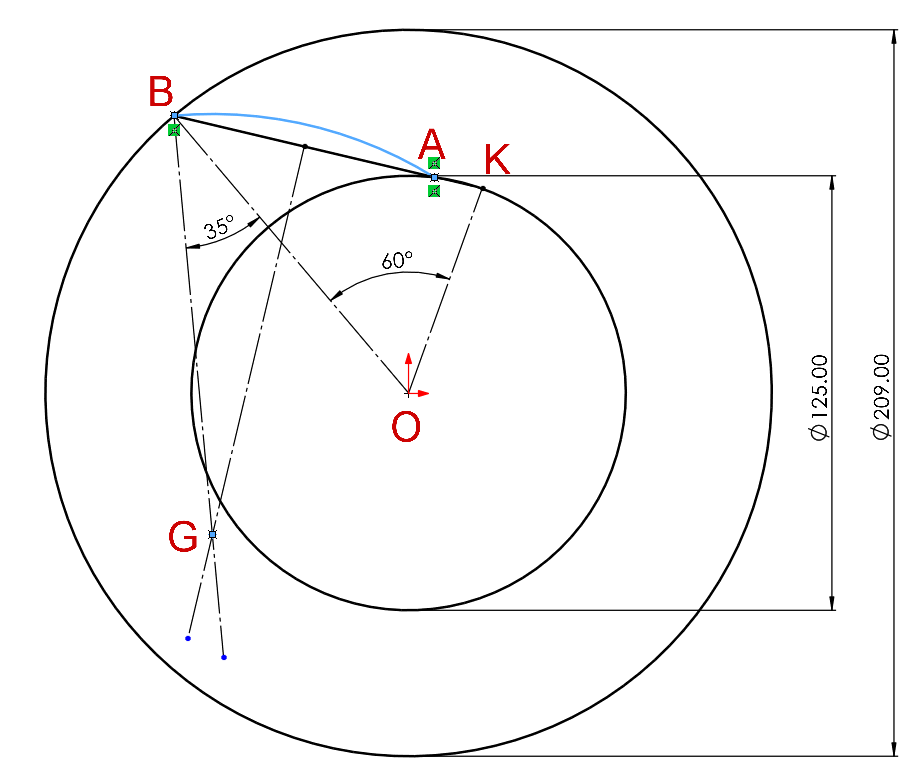
\includegraphics[width=0.94\linewidth,height=0.33\textheight,keepaspectratio]{figures/rId14.png}

\caption{Single arc construction using the perpendicular bisector and center G.}\end{figure}

To check the constructed arc, extend both ends and measure their angles relative to the circle tangents. As shown below, the source obtains the specified inlet and outlet angles, $\beta'_1$ and $\beta'_2$.

\begin{figure}[H]\centering

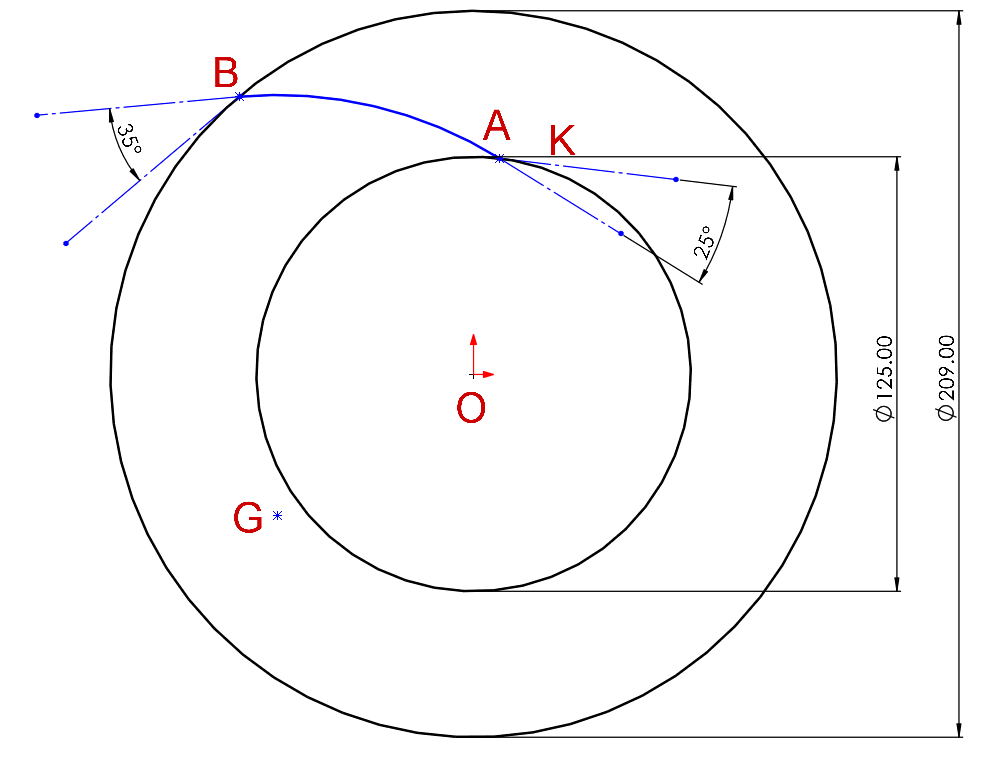
\includegraphics[width=0.94\linewidth,height=0.33\textheight,keepaspectratio]{figures/rId15.png}

\caption{Checking the inlet and outlet angles of the single arc profile.}\end{figure}

Six blades are required. Use the Circular Sketch Pattern tool in SolidWorks to repeat the arc five more times.

\begin{figure}[H]\centering

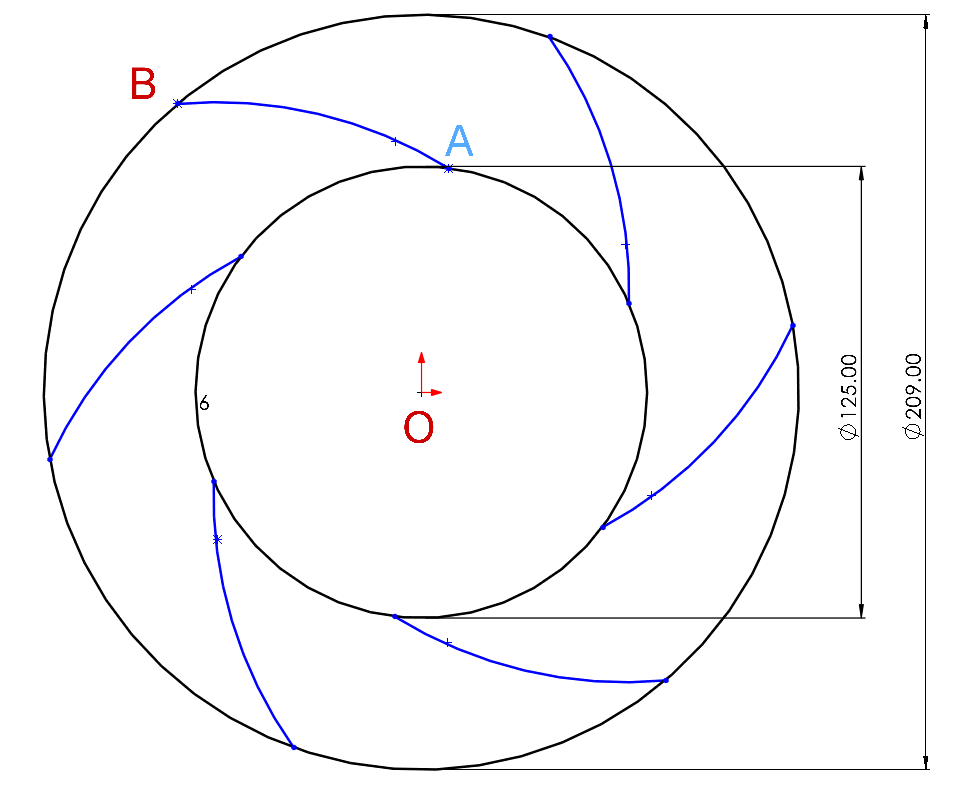
\includegraphics[width=0.94\linewidth,height=0.33\textheight,keepaspectratio]{figures/rId16.png}

\caption{Six blade profiles generated with Circular Sketch Pattern.}\end{figure}

The following drawing also shows the inlet and outlet angles used in the construction.

\begin{figure}[H]\centering

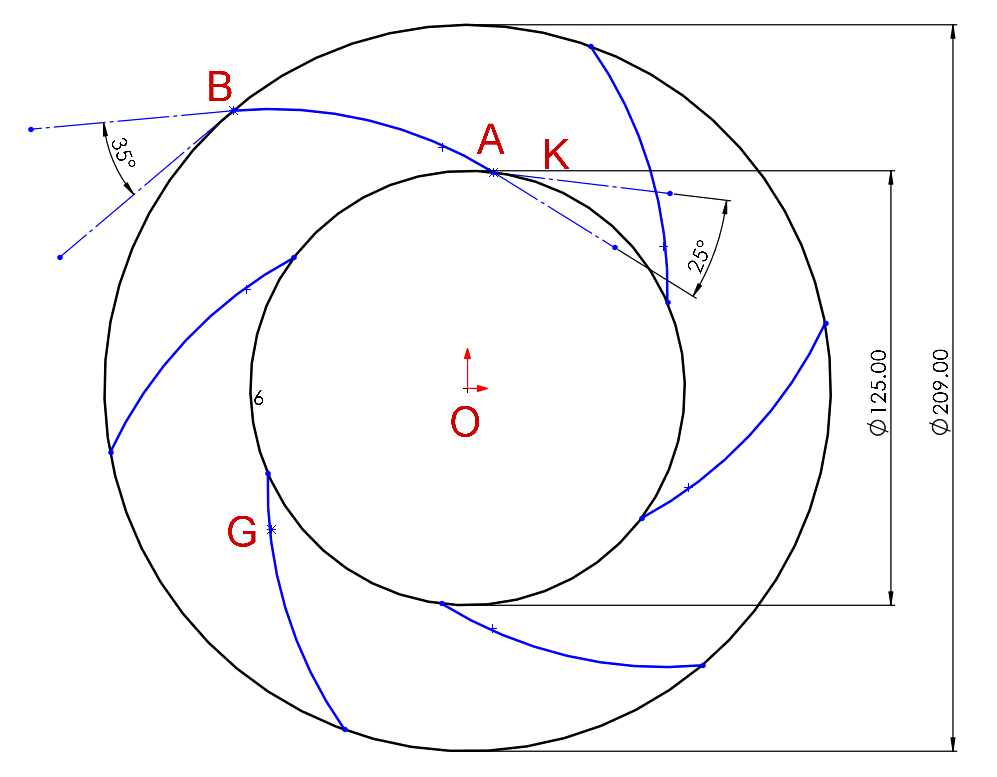
\includegraphics[width=0.94\linewidth,height=0.33\textheight,keepaspectratio]{figures/rId17.png}

\caption{Single arc blade construction with angle checks.}\end{figure}

\subsubsection{Double arc method}

To improve flow guidance, the blade is divided into two sections. The source calls the intermediate radius $R_m$ the geometric mean of the radii and defines it using the following expression:

\[R_m=\sqrt{\frac{R_1^2+R_2^2}{2}}=86.1\ \mathrm{mm}.\]

With linear interpolation, the blade angle at the intermediate point is $\beta_m=30^\circ$.

The first, inner arc extends from radius 62.5 mm at an angle of $25^\circ$ to radius 86.1 mm at an angle of $30^\circ$. The source calculates its radius as $R_{\mathrm{arc1}}=97.7$ mm.

The second, outer arc extends from radius 86.1 mm at $30^\circ$ to radius 104.5 mm at $35^\circ$. Its reported radius is $R_{\mathrm{arc2}}=159.1$ mm.

\paragraph{Construction procedure}

First, calculate $\delta$ using the procedure in the course's impeller design video:

\[\delta=D_1\sin\beta'_1=125\sin25^\circ=52.827\ \mathrm{mm}.\]

Draw a circle of diameter $\delta$ centered at $O$, in addition to the two principal circles.

\begin{figure}[H]\centering

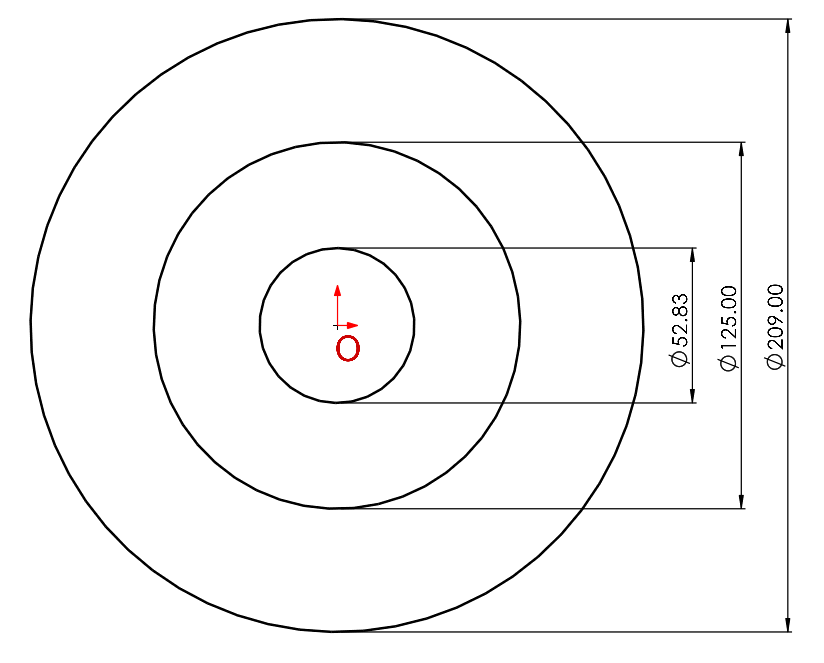
\includegraphics[width=0.94\linewidth,height=0.33\textheight,keepaspectratio]{figures/rId18.png}

\caption{Auxiliary circle of diameter delta for the double arc construction.}\end{figure}

Mark six points on the inner circle, and from each point draw a tangent to the circle of diameter $\delta$.

\begin{figure}[H]\centering

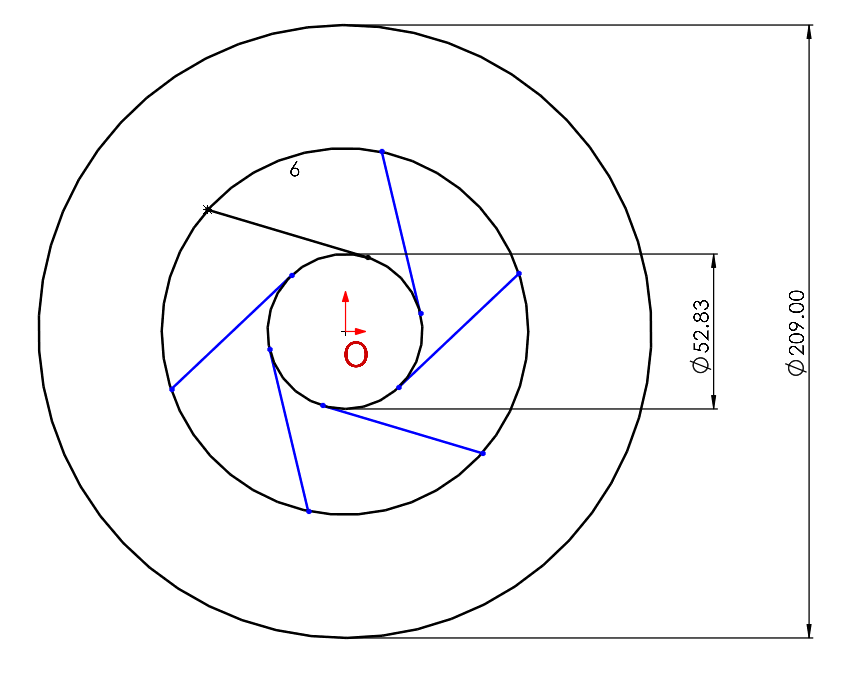
\includegraphics[width=0.94\linewidth,height=0.33\textheight,keepaspectratio]{figures/rId19.png}

\caption{Tangents drawn from the inlet circle to the auxiliary circle.}\end{figure}

Using the tangent lengths as radii and the corresponding tangency points on the smallest circle as centers, draw circular curves. Continue each curve until it meets the extension of the next tangent. Each resulting segment forms part of the complete blade profile.

\begin{figure}[H]\centering

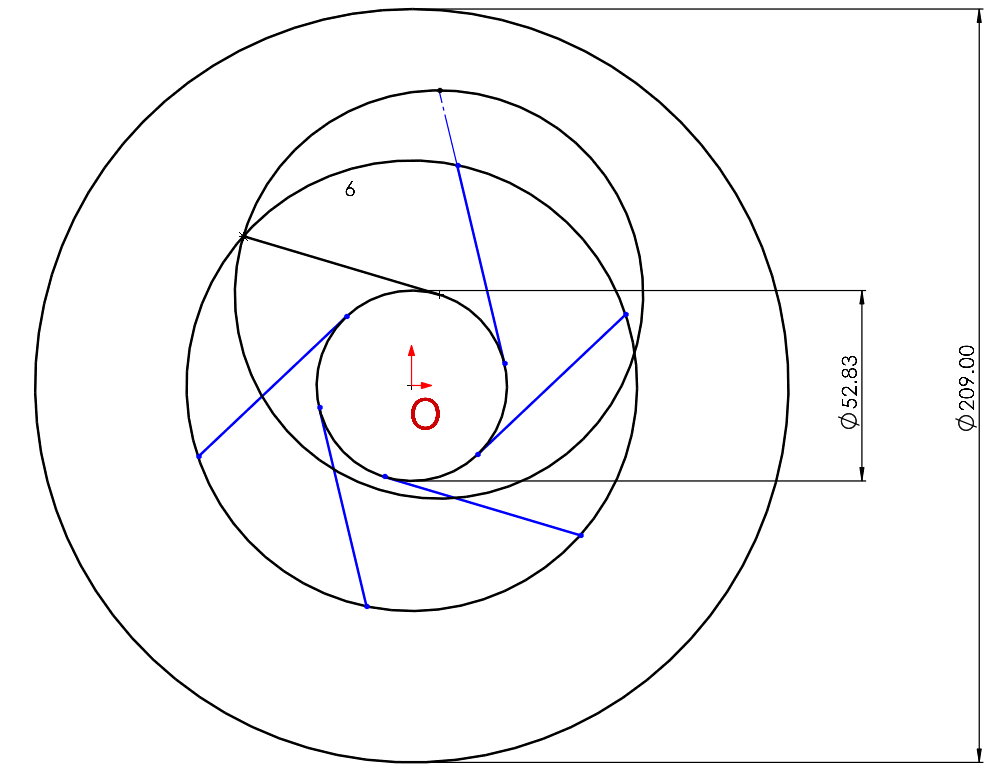
\includegraphics[width=0.94\linewidth,height=0.33\textheight,keepaspectratio]{figures/rId20.png}

\caption{Construction of the initial curved segments.}\end{figure}

Trim the unused portions of the circles.

\begin{figure}[H]\centering

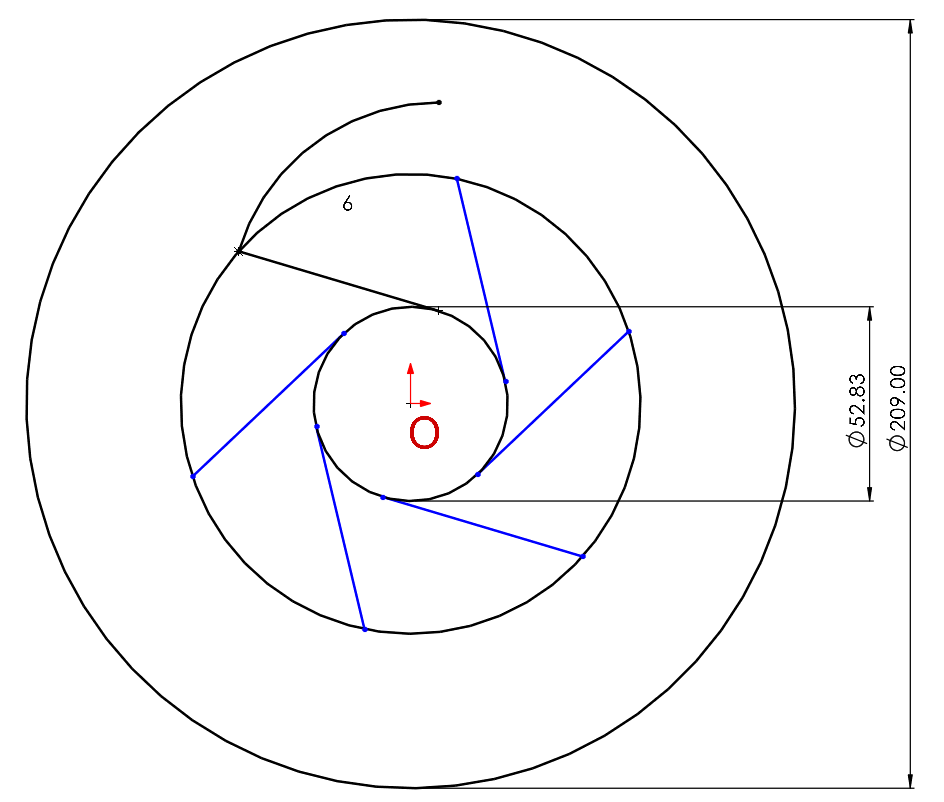
\includegraphics[width=0.94\linewidth,height=0.33\textheight,keepaspectratio]{figures/rId21.png}

\caption{Initial blade segments after trimming the auxiliary circles.}\end{figure}

The partial blade profile is now visible. To continue the construction, determine the remaining arc radius $\rho$ using

\[\rho=\frac{1}{2}\frac{R_2^2-R_F^2}{R_2\cos\beta'_2-R_F\cos\beta'_F}.\]

Here, $R_F$ is the distance from the impeller center to the end of the constructed curve. The source describes the relevant angle as the angle between $R_F$ and the line joining the curve endpoint to the first point on the $\delta$ circle, but labels it $\beta'_2$ in this sentence. On that connecting line, locate point $G$ a distance $\rho$ from the curve endpoint, then draw a circle centered at $G$ with radius $\rho$ to join the curve to the outer circle. See the editorial note on the angle-label inconsistency.

\begin{figure}[H]\centering

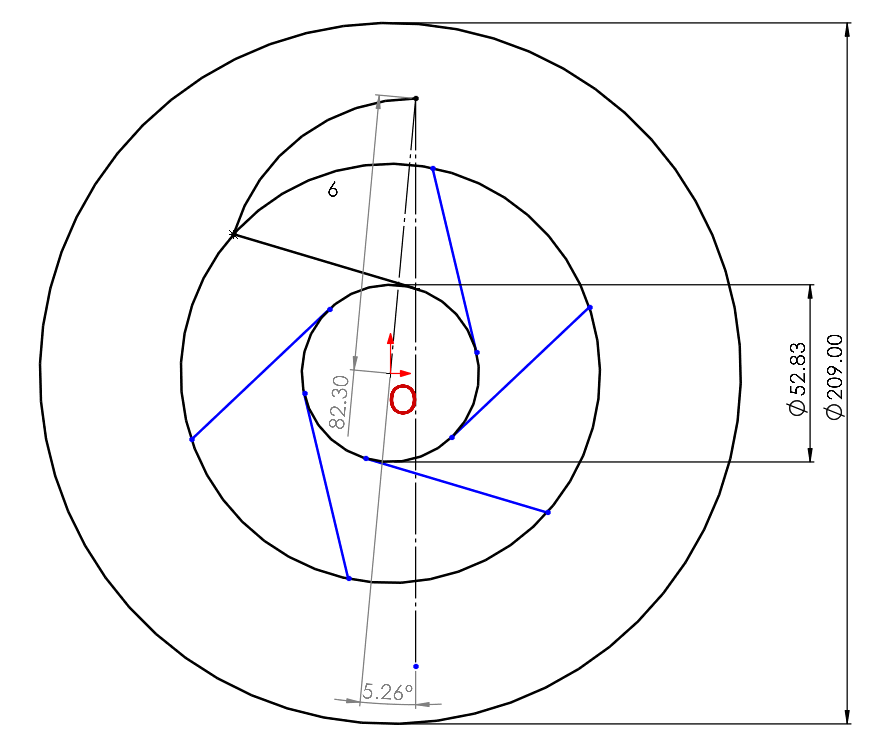
\includegraphics[width=0.94\linewidth,height=0.33\textheight,keepaspectratio]{figures/rId22.png}

\caption{Determination of the intermediate endpoint and connecting arc.}\end{figure}

From the SolidWorks drawing above, the unknown quantities are obtained as

\[R_F=82.30\ \mathrm{mm},\]

\[\beta'_F=5.26^\circ.\]

\[\rho=\frac{1}{2}\frac{104.5^2-82.30^2}{104.5\cos35^\circ-82.30\cos5.26^\circ}\]

\[\Longrightarrow\quad\rho=568.39\ \mathrm{mm}.\]

Thus, locate the center a distance $\rho$ from the end of the existing curve and draw a circle of radius $\rho$.

\begin{figure}[H]\centering

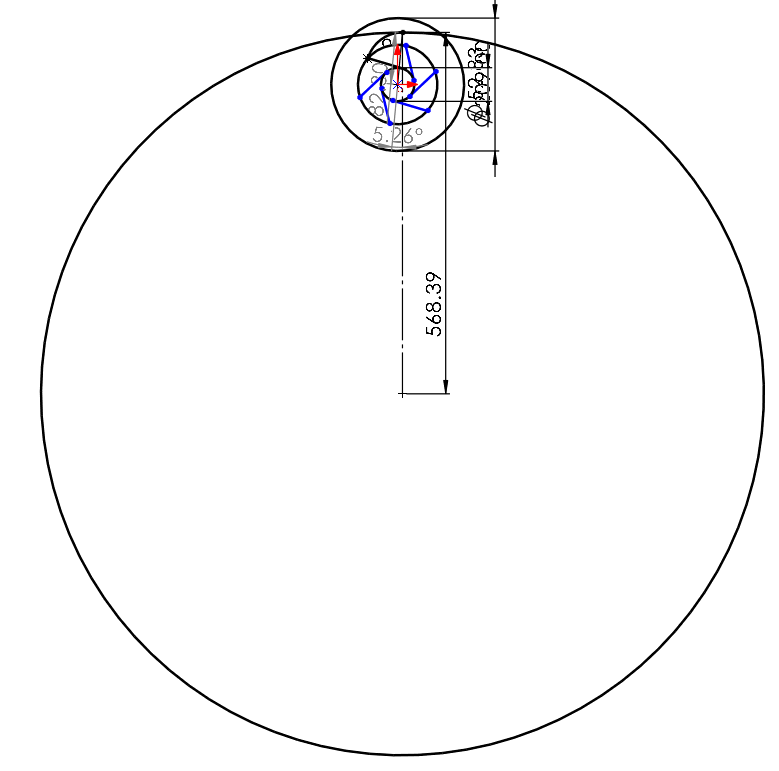
\includegraphics[width=0.94\linewidth,height=0.33\textheight,keepaspectratio]{figures/rId23.png}

\caption{Construction of the final arc of radius 568.39 mm.}\end{figure}

Trim the extra portions and check the inlet and outlet angles.

\begin{figure}[H]\centering

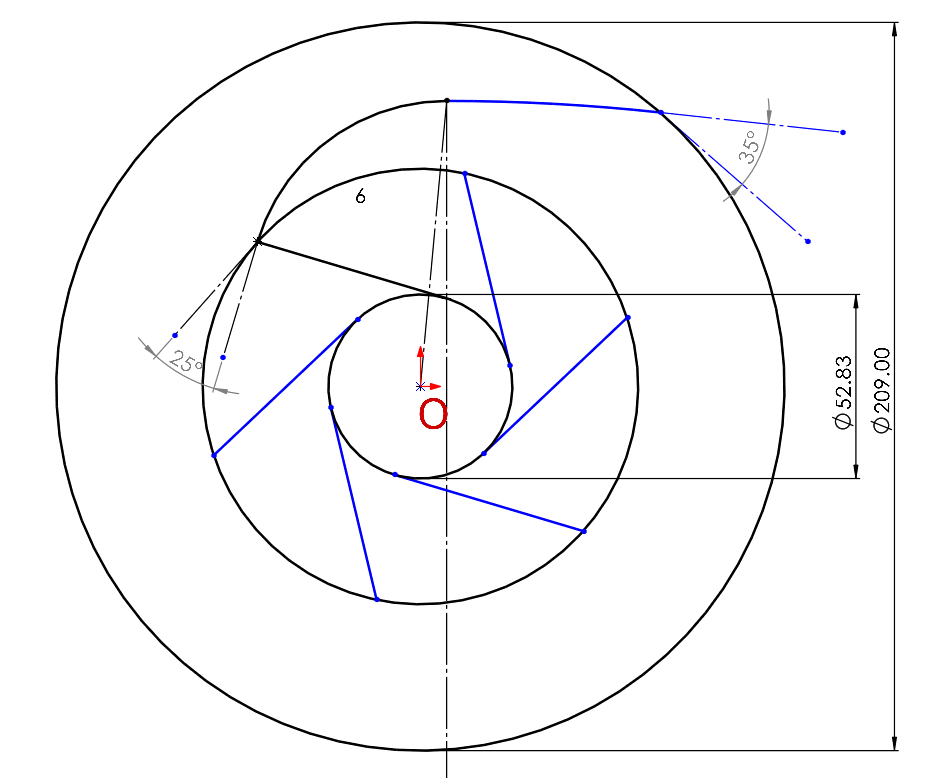
\includegraphics[width=0.94\linewidth,height=0.33\textheight,keepaspectratio]{figures/rId24.png}

\caption{Angle checks after trimming the final connecting arc.}\end{figure}

The drawing shows the specified inlet and outlet angles. The blade profiles are then redrawn without the auxiliary construction geometry.

\begin{figure}[H]\centering

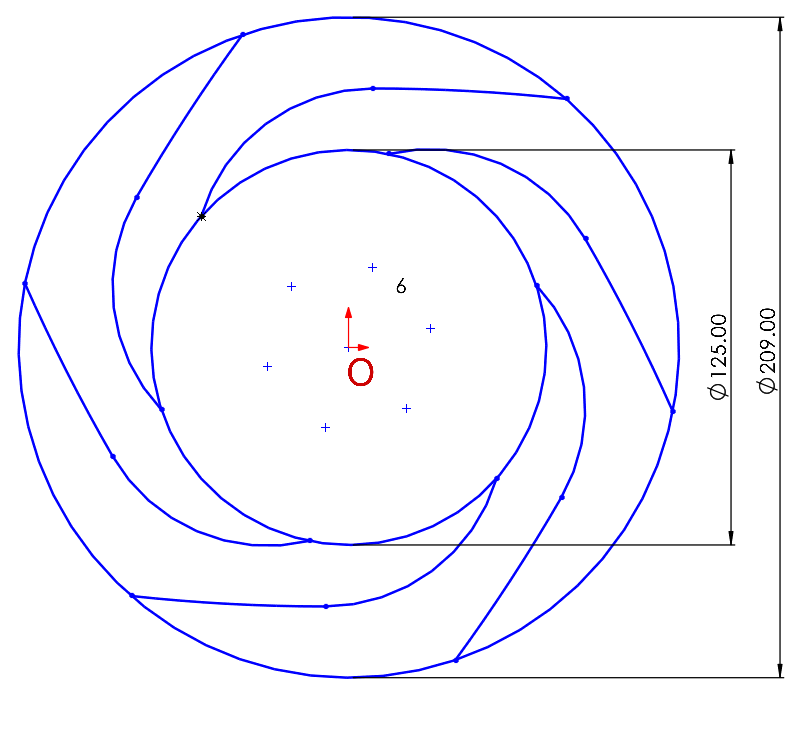
\includegraphics[width=0.94\linewidth,height=0.33\textheight,keepaspectratio]{figures/rId25.png}

\caption{Completed blade profiles without construction lines.}\end{figure}

\begin{table}[H]\centering\small
\caption{Blade metal and relative-flow angles reported in Phase One.}
\begin{tabular}{p{0.32\linewidth}cp{0.46\linewidth}}\toprule
Parameter & Value & Description\\\midrule
Inlet metal angle $\beta'_1$ & $25^\circ$ & Blade construction angle, including $5.5^\circ$ incidence.\\
Outlet metal angle $\beta'_2$ & $35^\circ$ & Outlet construction angle used to draw the blade arc.\\
Inlet flow angle $\beta_1$ & $19.5^\circ$ & Relative inlet direction from the velocity triangle.\\
Outlet flow angle $\beta_2$ & $15.6^\circ$ & Actual relative outlet direction including slip.\\\bottomrule
\end{tabular}\end{table}

\FloatBarrier\section{Phase Two Impeller Modeling in CFturbo}

After the initial geometric design in Phase One, Phase Two addresses the three-dimensional modeling and detailed simulation of the 100-200 pump impeller in CFturbo. The source describes the software as converting the extracted operating parameters and dimensions into a detailed CAD model and predicting the pump's fluid behavior.

\subsection{Entering the duty point}

The CFturbo workflow starts by defining the pump operating conditions. The Phase One values for the best efficiency point are entered into the software:

Working fluid: water at the reference temperature, with a density of $1000\ \mathrm{kg/m^3}$.

Rotational speed: $N=1450$ rpm.

Volumetric flow rate: $Q=125\ \mathrm{m^3/h}$, equivalent to approximately $0.0347\ \mathrm{m^3/s}$.

Developed head: $H=13.5$ m.

From these inputs, CFturbo calculates the specific speed and identifies the turbomachine as a radial centrifugal pump.

\begin{figure}[H]\centering

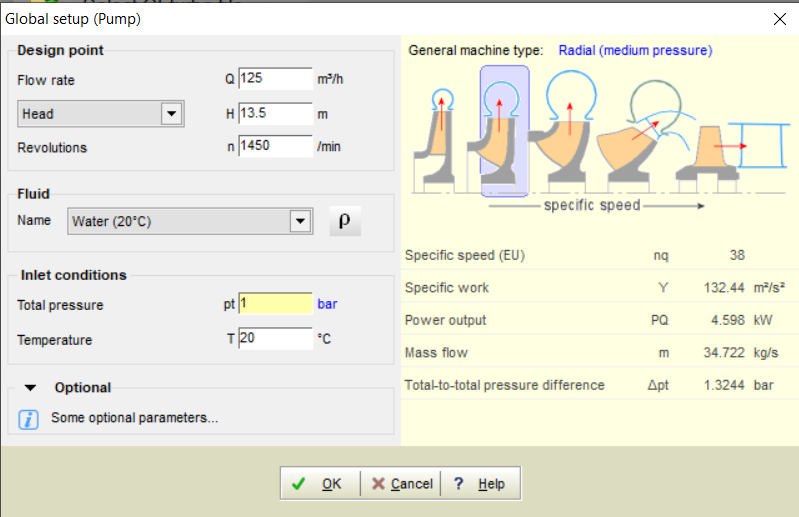
\includegraphics[width=0.94\linewidth,height=0.33\textheight,keepaspectratio]{figures/rId26.png}

\caption{CFturbo global setup at the adopted duty point.}\end{figure}

The proposed machine type is shown as \texttt{Radial (medium pressure)}. The hydraulic efficiency was taken as 90\% in Phase One, so the same value is entered here.

\begin{figure}[H]\centering

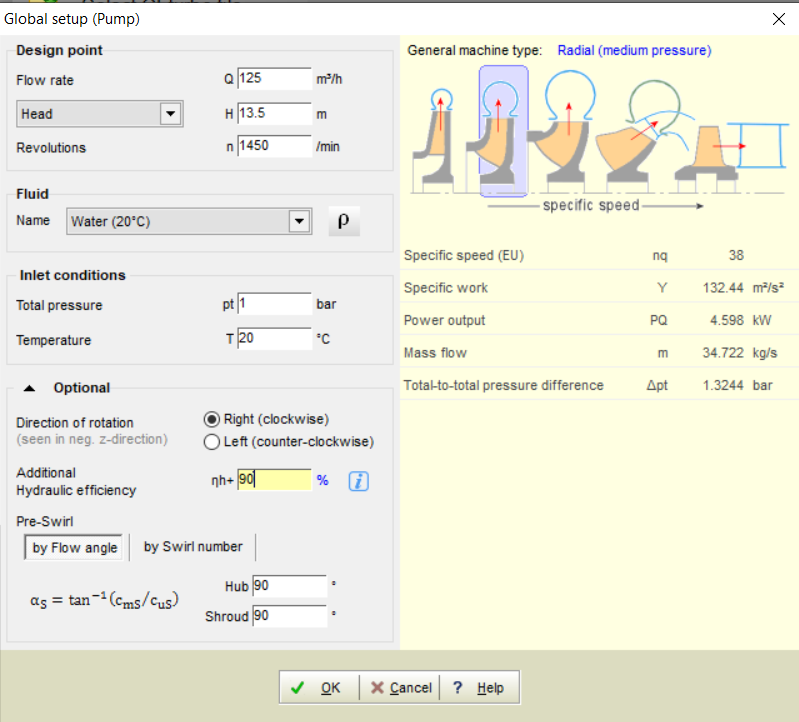
\includegraphics[width=0.94\linewidth,height=0.33\textheight,keepaspectratio]{figures/rId27.png}

\caption{Duty point and efficiency settings.}\end{figure}

From Add Component, choose Radial/Mixed-flow Impeller. Then select the options shown in the Setup tab of Main Dimensions. The source leaves Unshrouded unchecked so that the impeller has a front shroud, explaining this choice in terms of the water-pump application. Splitter Blades is also left unchecked; the source states that the pump size does not require additional outlet flow guidance of that type.

\begin{figure}[H]\centering

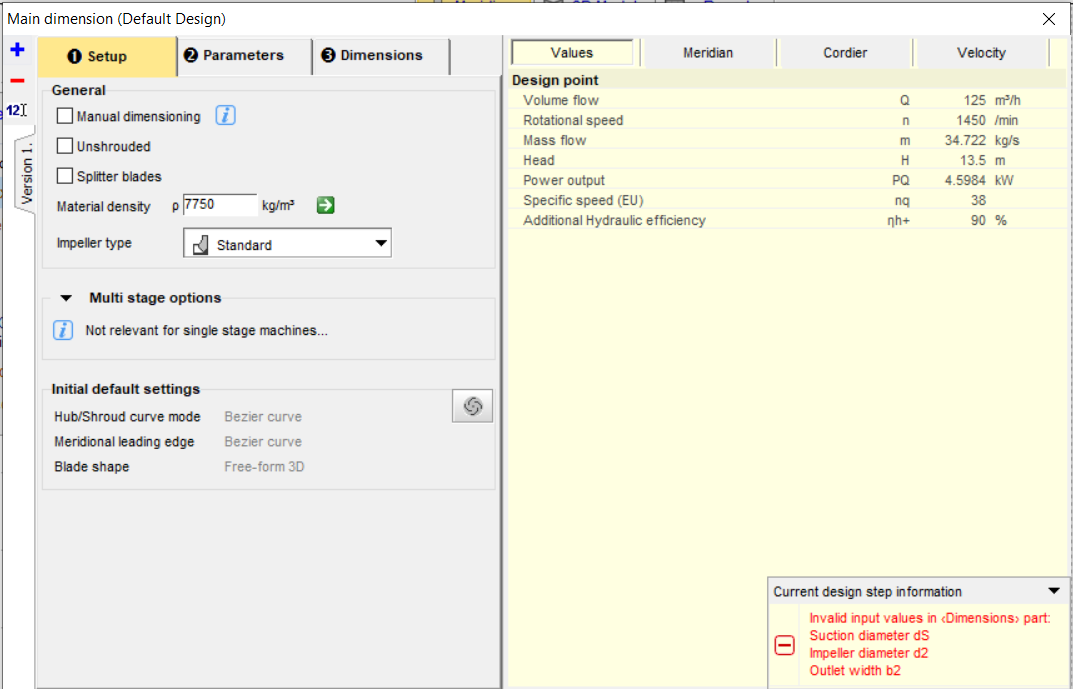
\includegraphics[width=0.94\linewidth,height=0.33\textheight,keepaspectratio]{figures/rId28.png}

\caption{Radial impeller setup options.}\end{figure}

In the Parameters tab, the default values are initially retained because they lie in suitable regions of the displayed parameter curves. The manually calculated value of $b_2/D_2$, however, falls outside the indicated recommended region and is considered unsuitable.

\begin{figure}[H]\centering

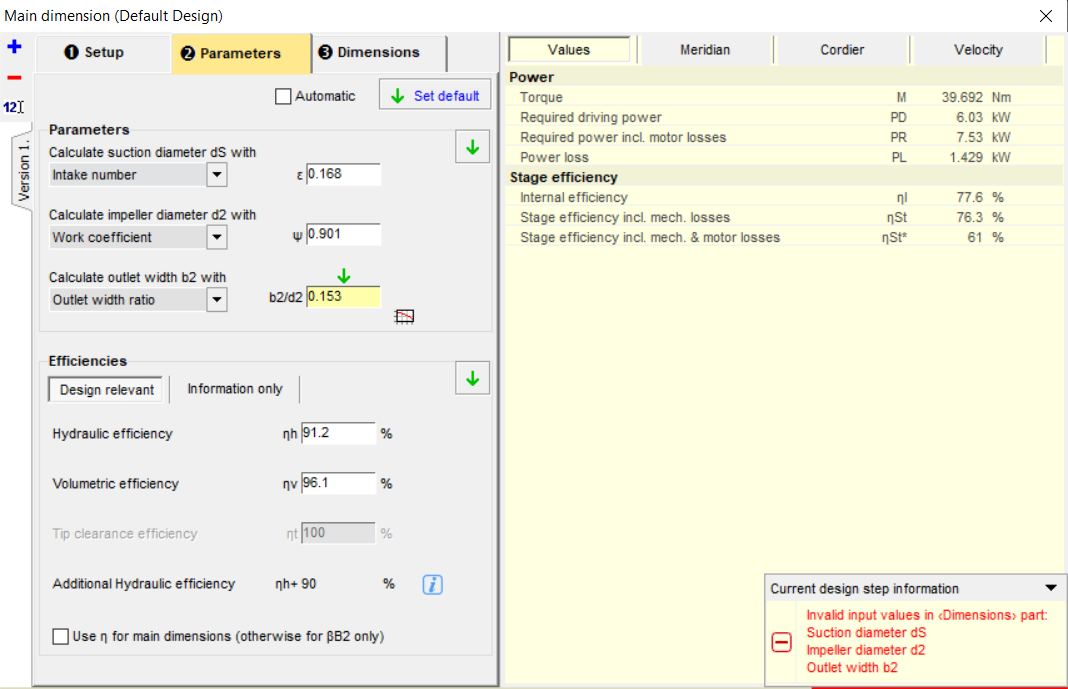
\includegraphics[width=0.94\linewidth,height=0.33\textheight,keepaspectratio]{figures/rId29.png}

\caption{Initial parameter choices and warning messages.}\end{figure}

\begin{figure}[H]\centering

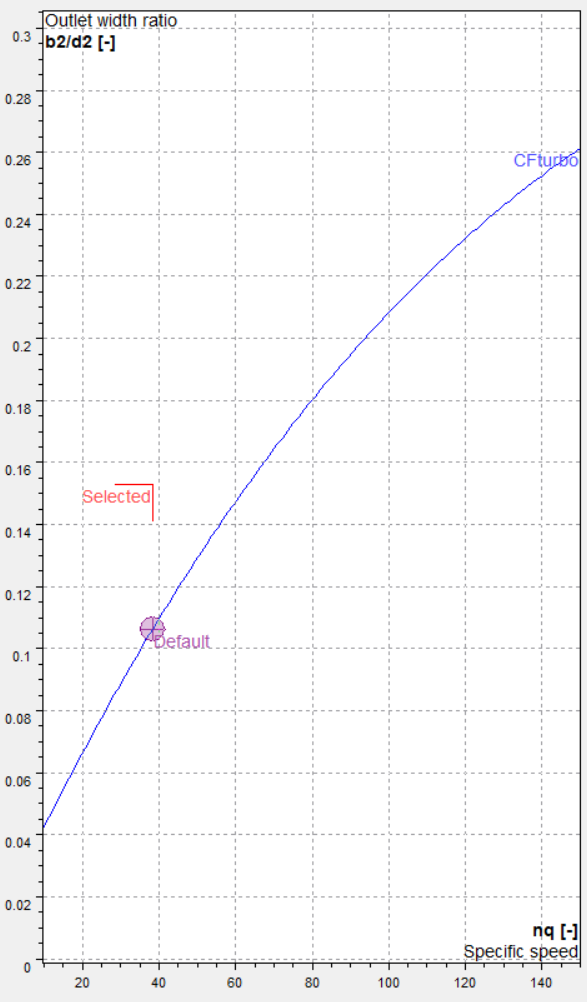
\includegraphics[width=0.94\linewidth,height=0.33\textheight,keepaspectratio]{figures/rId30.png}

\caption{Parameter chart for the outlet width ratio.}\end{figure}

The $b_2/D_2$ parameter is therefore also returned to its default value.

\begin{figure}[H]\centering

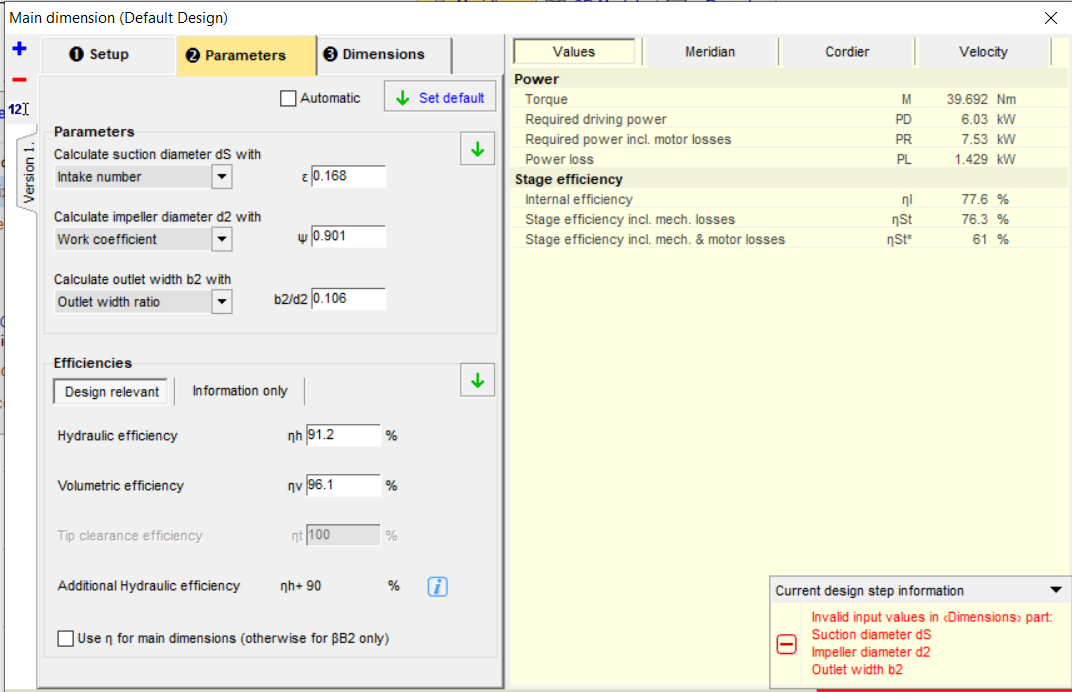
\includegraphics[width=0.94\linewidth,height=0.33\textheight,keepaspectratio]{figures/rId31.png}

\caption{Parameters after restoring the default width ratio.}\end{figure}

In the Dimensions tab, select the shaft specification. The Pumpiran catalog lists Ck45 steel as the shaft material for the 100-200 pump.

\begin{figure}[H]\centering

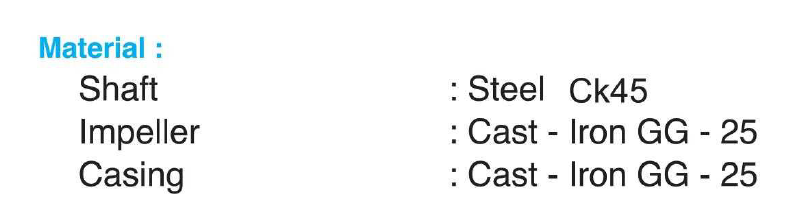
\includegraphics[width=0.94\linewidth,height=0.33\textheight,keepaspectratio]{figures/rId32.png}

\caption{Catalog material specification for the shaft, impeller, and casing.}\end{figure}

The corresponding allowable stress is selected.

\begin{figure}[H]\centering

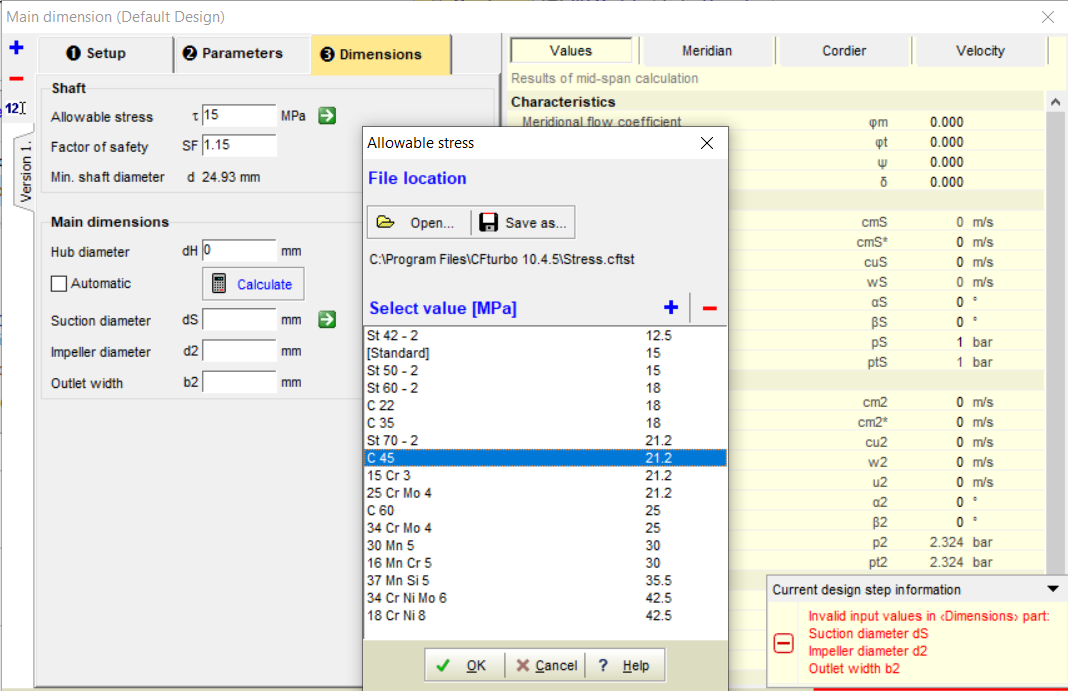
\includegraphics[width=0.94\linewidth,height=0.33\textheight,keepaspectratio]{figures/rId33.png}

\caption{Selection of allowable shaft stress.}\end{figure}

The factor of safety is increased to 1.2, and the hub diameter is set to 45 mm.

\begin{figure}[H]\centering

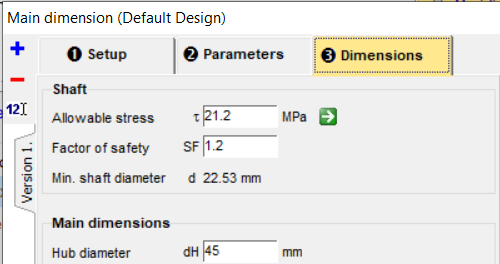
\includegraphics[width=0.94\linewidth,height=0.33\textheight,keepaspectratio]{figures/rId34.png}

\caption{Shaft safety factor and hub diameter settings.}\end{figure}

Press Calculate to let CFturbo determine the diameter and width values.

\subsection{Meridional design}

This step defines the impeller's longitudinal section. The source lists the Phase One dimensions as geometric constraints to enter into the software:

\begin{table}[H]\centering\small
\caption{Phase One dimensions listed as intended CFturbo inputs in the source.}
\begin{tabular}{llp{0.5\linewidth}}\toprule
Dimension & Symbol & Reported value\\\midrule
Shaft diameter & $d_s$ & 32 mm; hub diameter 45 mm\\
Impeller eye diameter & $D_1$ & 125 mm\\
Impeller outlet diameter & $D_2$ & 209 mm\\
Inlet blade width & $b_1$ & 32 mm\\
Outlet blade width & $b_2$ & 32 mm\\\bottomrule
\end{tabular}\end{table}

The dimensions initially calculated by CFturbo are shown below.

\begin{figure}[H]\centering

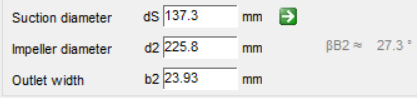
\includegraphics[width=0.94\linewidth,height=0.33\textheight,keepaspectratio]{figures/rId35.png}

\caption{Initial main dimensions proposed by CFturbo.}\end{figure}

The source states that only the shaft diameter differs substantially from the Phase One values and proposes adjusting it using the standard diameter in the catalog. The following figures and the DN designation refer to the suction connection; this terminology conflict is addressed in the editorial appendix.

\begin{figure}[H]\centering

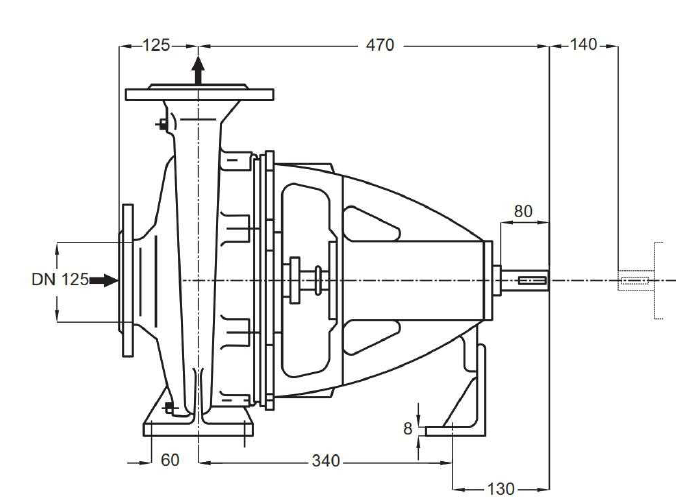
\includegraphics[width=0.94\linewidth,height=0.33\textheight,keepaspectratio]{figures/rId36.png}

\caption{Catalog drawing showing the DN 125 suction connection.}\end{figure}

From the Pumpiran catalog drawing above, the source identifies DN 125 as the standard nominal diameter.

\begin{figure}[H]\centering

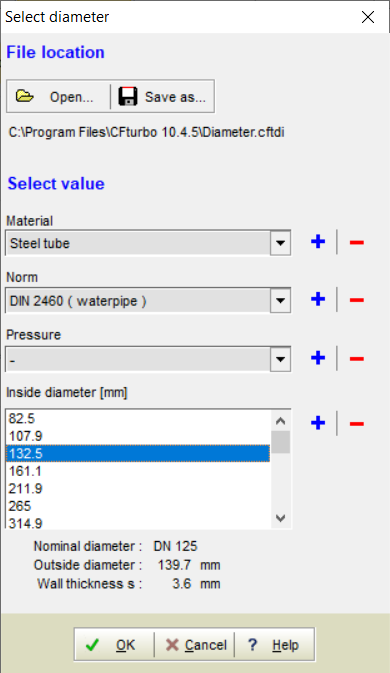
\includegraphics[width=0.94\linewidth,height=0.33\textheight,keepaspectratio]{figures/rId37.png}

\caption{Selection of a standard suction diameter.}\end{figure}

The resulting parameter values are shown below.

\begin{figure}[H]\centering

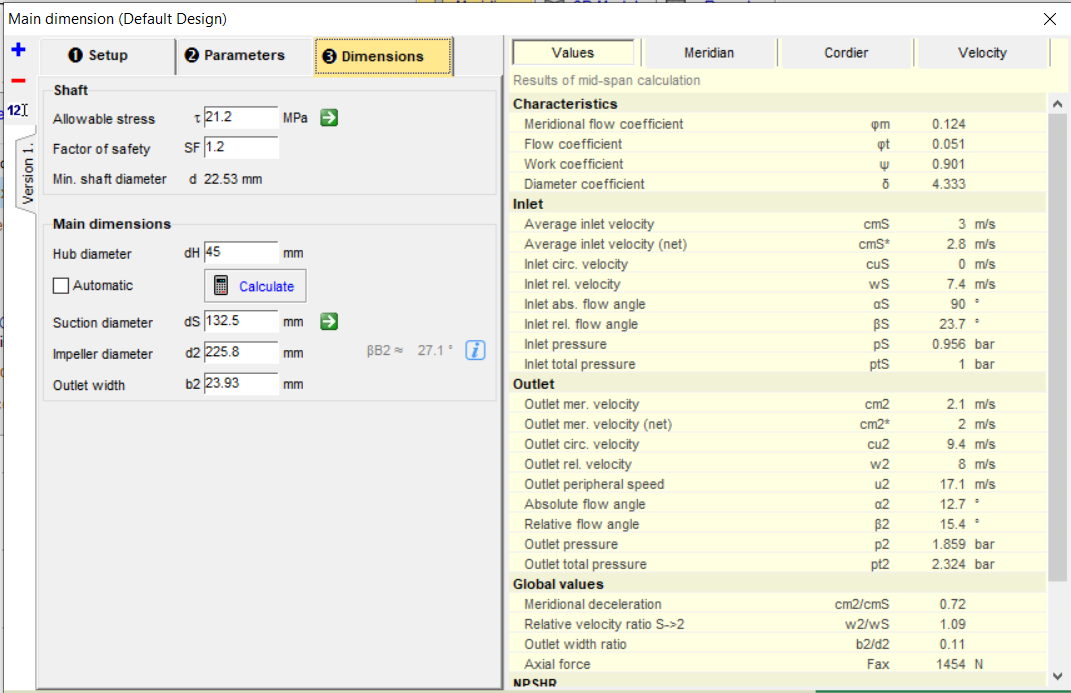
\includegraphics[width=0.94\linewidth,height=0.33\textheight,keepaspectratio]{figures/rId38.png}

\caption{Main dimension settings after adjustment.}\end{figure}

The Cordier diagram available in the same dialog places the selected design point between the two red curves. The source treats this as an indication that the design is acceptable.

\begin{figure}[H]\centering

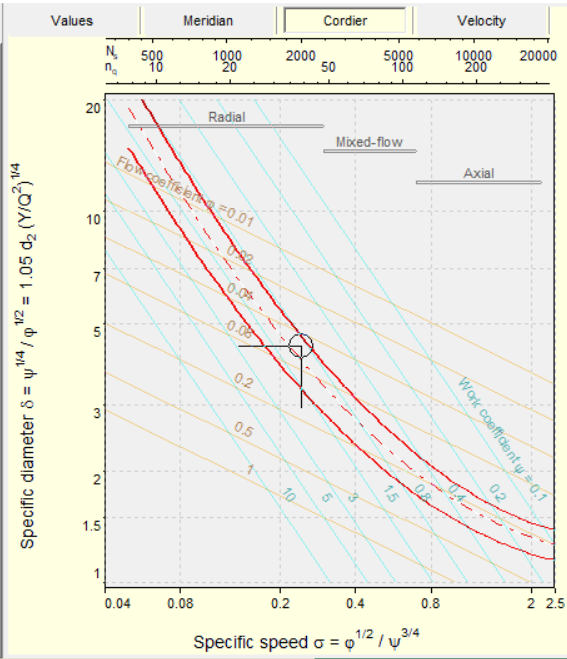
\includegraphics[width=0.94\linewidth,height=0.33\textheight,keepaspectratio]{figures/rId39.png}

\caption{Cordier diagram for the selected operating point.}\end{figure}

The velocity triangles are shown below.

\begin{figure}[H]\centering

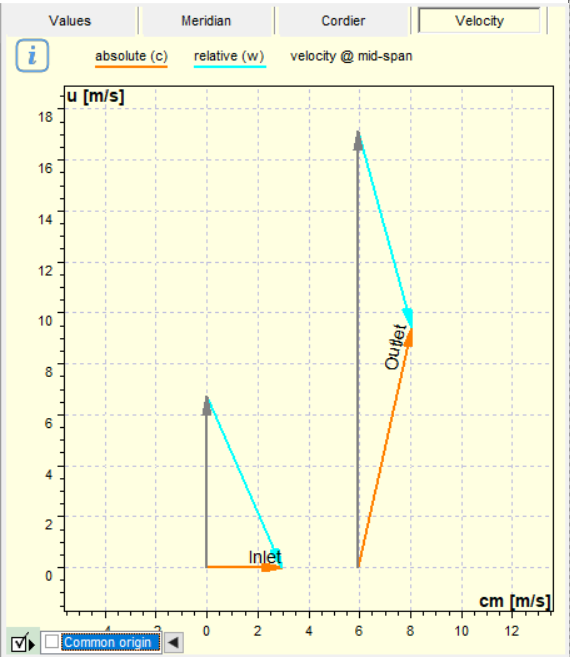
\includegraphics[width=0.94\linewidth,height=0.33\textheight,keepaspectratio]{figures/rId40.png}

\caption{CFturbo inlet and outlet velocity triangles.}\end{figure}

The impeller hub and shroud contours are adjusted using Bezier curves in CFturbo, aiming for a smooth variation of passage area and avoiding abrupt changes in velocity.

\begin{figure}[H]\centering

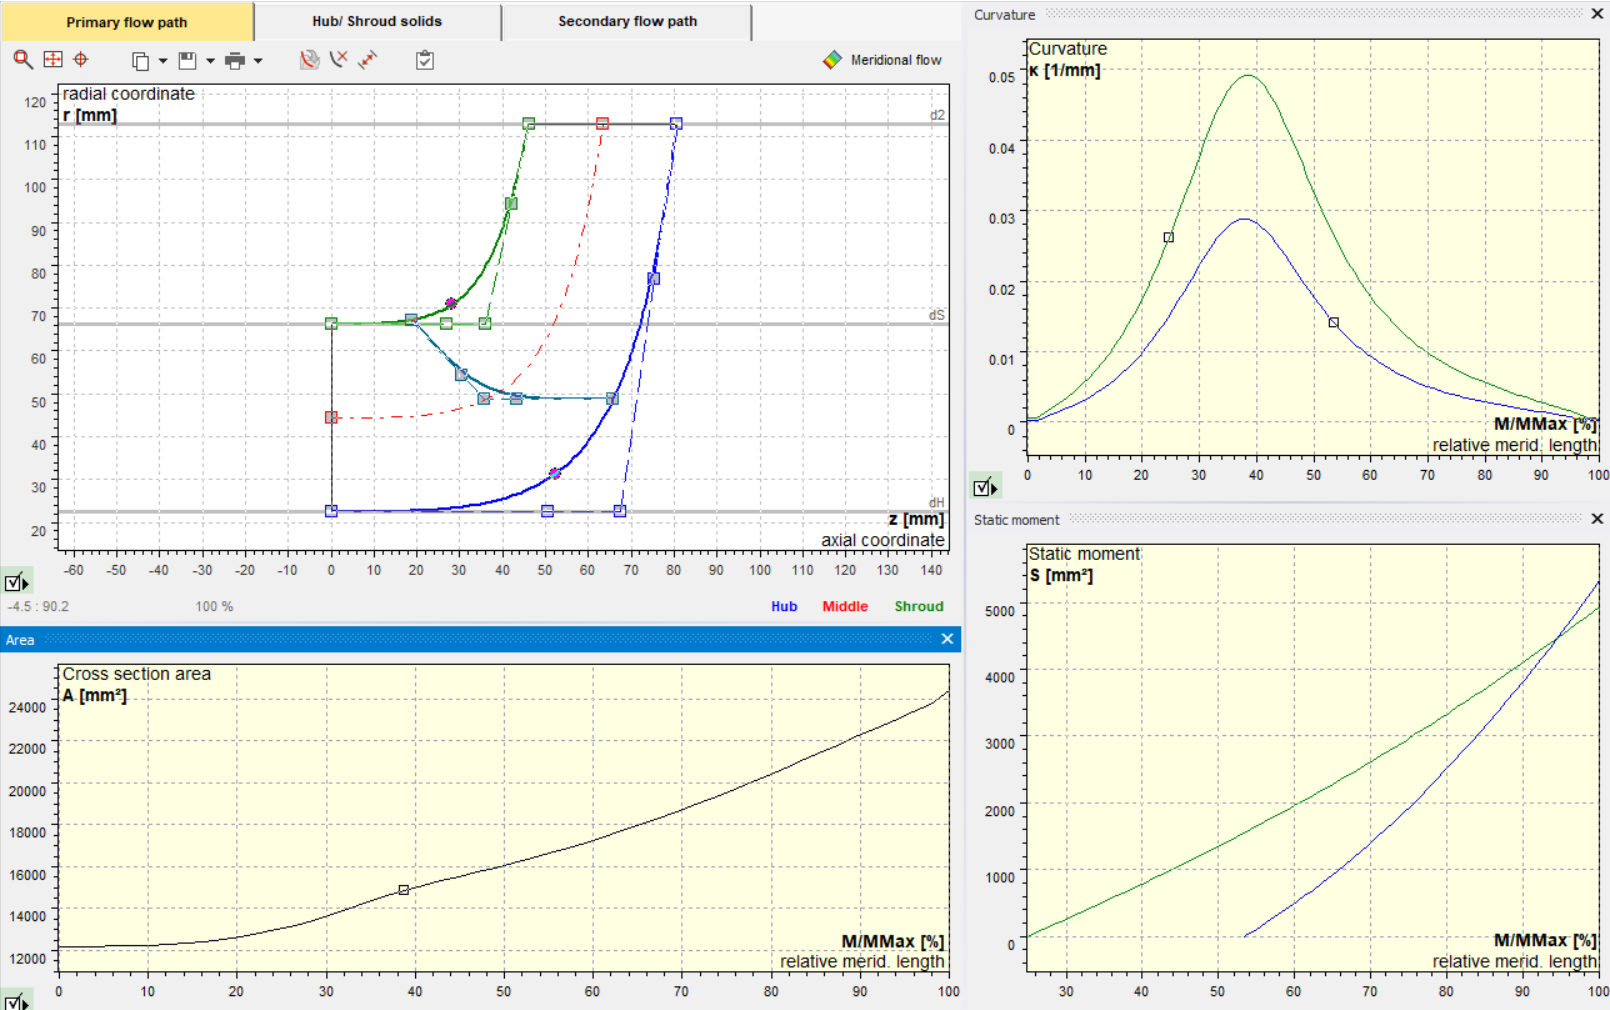
\includegraphics[width=0.94\linewidth,height=0.33\textheight,keepaspectratio]{figures/rId41.png}

\caption{Initial meridional contour and diagnostic plots.}\end{figure}

Alongside the meridional blade view, the software displays Curvature, Cross Section Area, and Static Moment plots. The source states that lower specific speed calls for a straighter meridional centerline, while higher specific speed allows a more concave profile, as in this design. The cross-sectional area curve should preferably be smooth, with no sudden jumps; the initial geometry already satisfies this visual criterion. The two static-moment curves should preferably be close to each other. Small adjustments to the Bezier control points improve this plot.

\begin{figure}[H]\centering

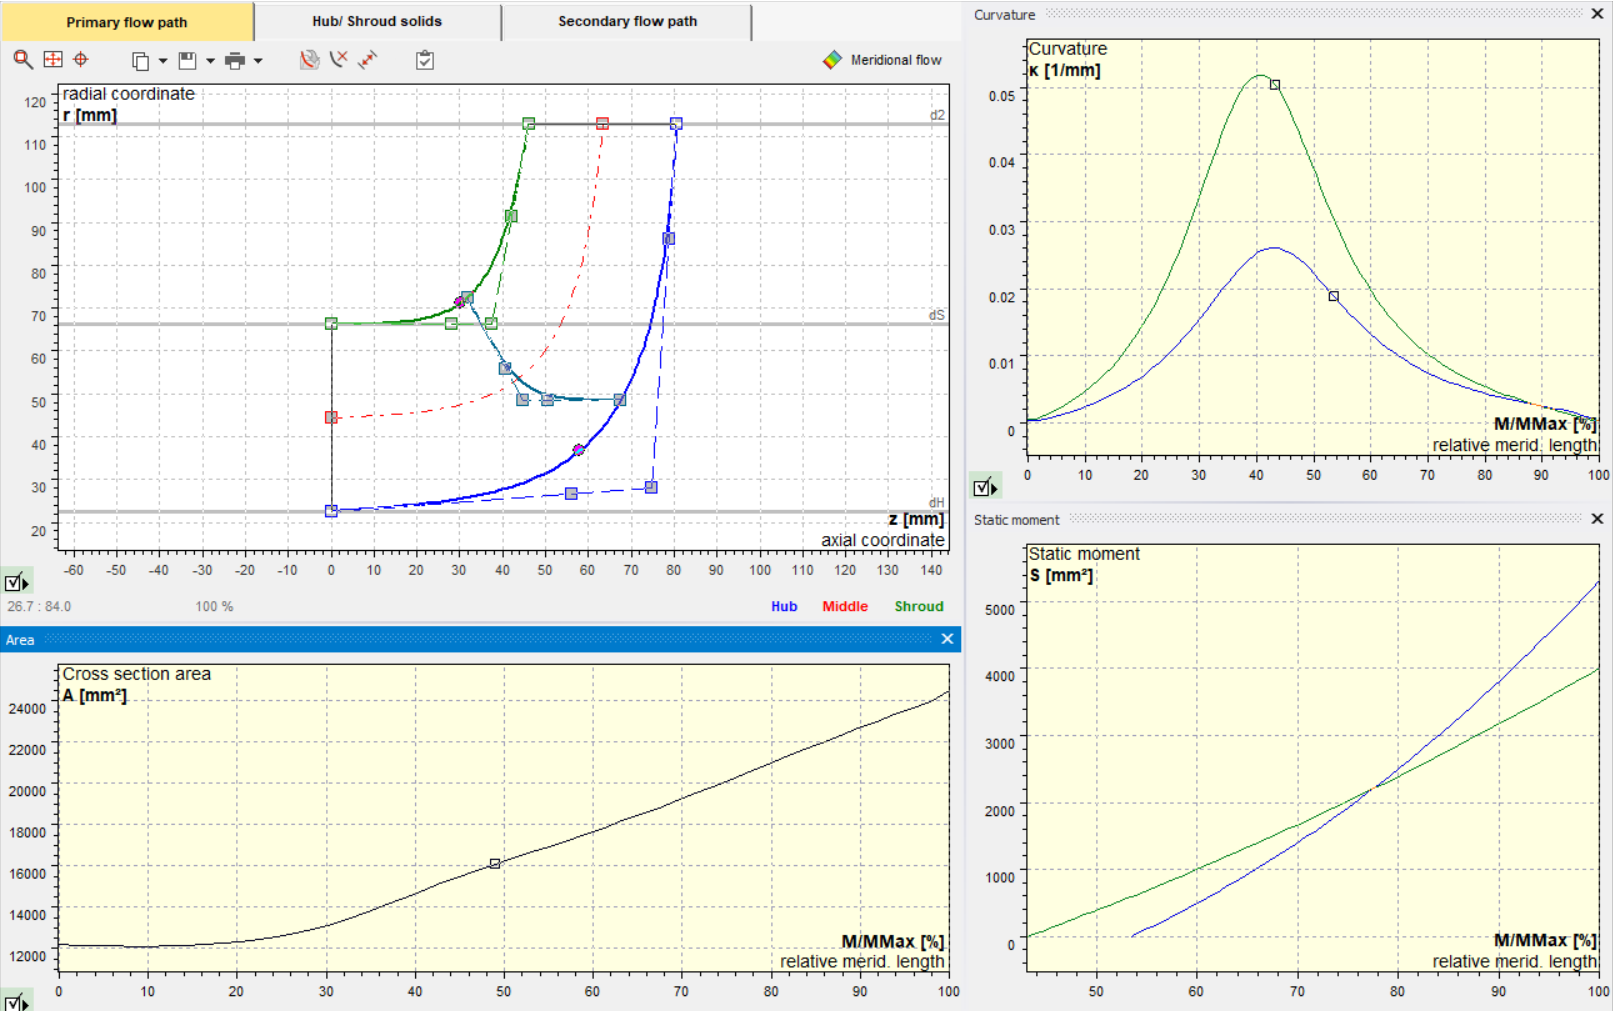
\includegraphics[width=0.94\linewidth,height=0.33\textheight,keepaspectratio]{figures/rId42.png}

\caption{Meridional diagnostic plots after adjusting the Bezier curves.}\end{figure}

The impeller is mounted on the shaft using a shaft-end nut. On the suction side, this nut occupies part of the inlet flow area. The source therefore extends the hub contour forward relative to the shroud contour, aiming to reduce the obstruction of the effective suction area and improve entry into the flow passage.

\begin{figure}[H]\centering

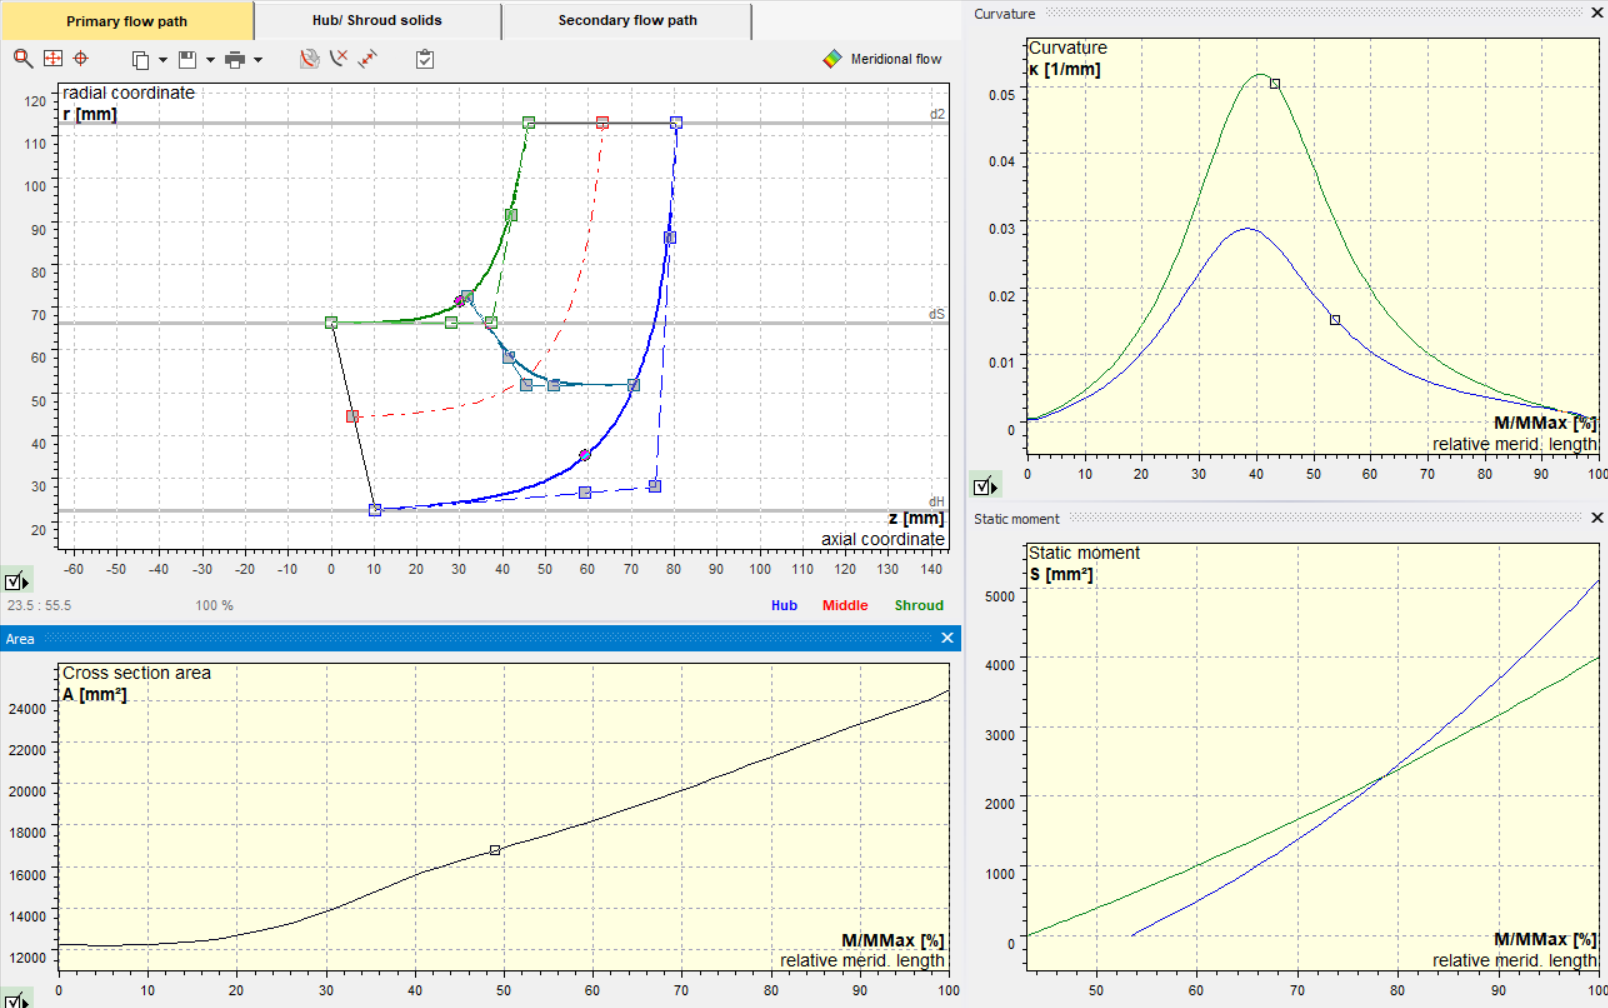
\includegraphics[width=0.94\linewidth,height=0.33\textheight,keepaspectratio]{figures/rId43.png}

\caption{Hub contour extended toward the inlet relative to the shroud.}\end{figure}

\subsection{Blade angles and thickness distribution}

This is identified as the principal blade-design step in CFturbo. The geometric angles calculated in Phase One are initially specified as follows:

Number of blades: six.

Inlet blade metal angle: $\beta'_1=25^\circ$.

Outlet blade metal angle: $\beta'_2=35^\circ$.

The blade-angle distributions from inlet to outlet on the hub and shroud surfaces are refined using CFturbo's conformal-mapping diagrams. The source also describes a gradual thickness distribution for the cast-iron blades, with a thinner leading edge to reduce incidence and blockage and a thicker trailing edge for mechanical strength.

With a specific speed of approximately 38, the source adopts the course recommendation to use Free-form 3D geometry above a specific speed of 15. Although this option is more expensive to manufacture than a two-dimensional blade, the source expects better efficiency and describes the choice as a tradeoff between efficiency and cost.

The proposed blade thickness range is 3.2--3.7 mm. A value of 3.4 mm is selected at the hub for both the leading and trailing edges, while 3.2 mm is selected at the shroud to create a spanwise thickness gradient. The source explains that this gradient facilitates removal from a casting mold compared with a uniformly thick blade. The blade count remains six, and Number of Spans is set to seven. The source treats this setting as a finer geometric subdivision rather than a change to the other design parameters. The remaining choices are shown below.

\begin{figure}[H]\centering

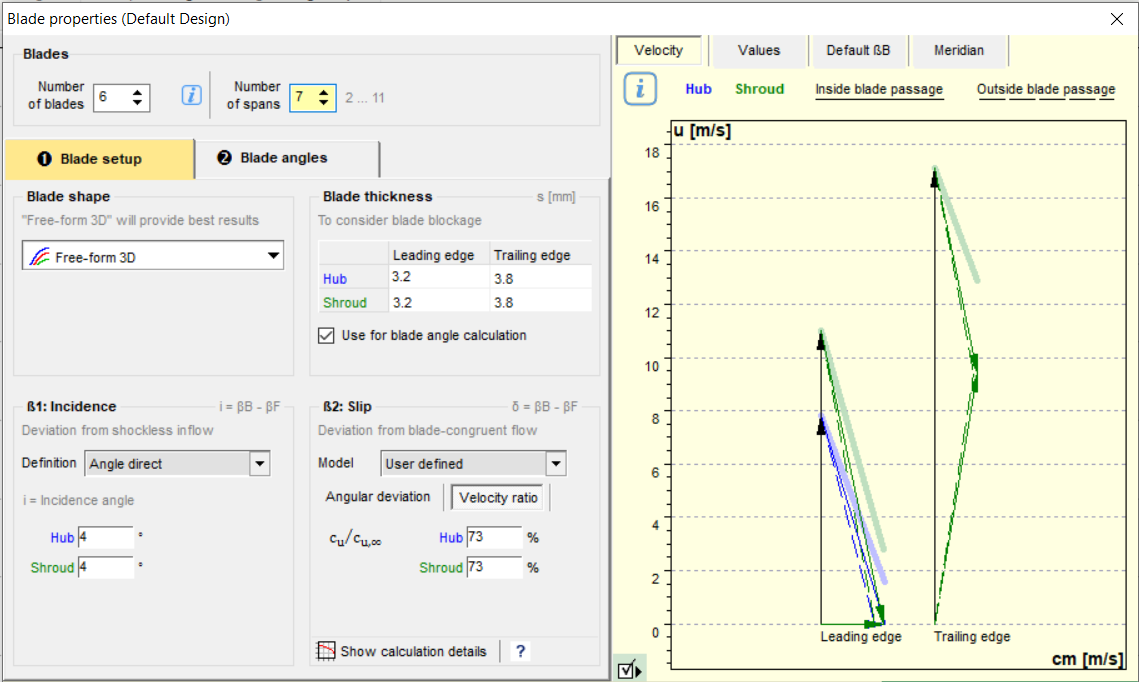
\includegraphics[width=0.94\linewidth,height=0.33\textheight,keepaspectratio]{figures/rId44.png}

\caption{Free-form three-dimensional blade properties.}\end{figure}

The blade angles are then selected automatically by the software.

\begin{figure}[H]\centering

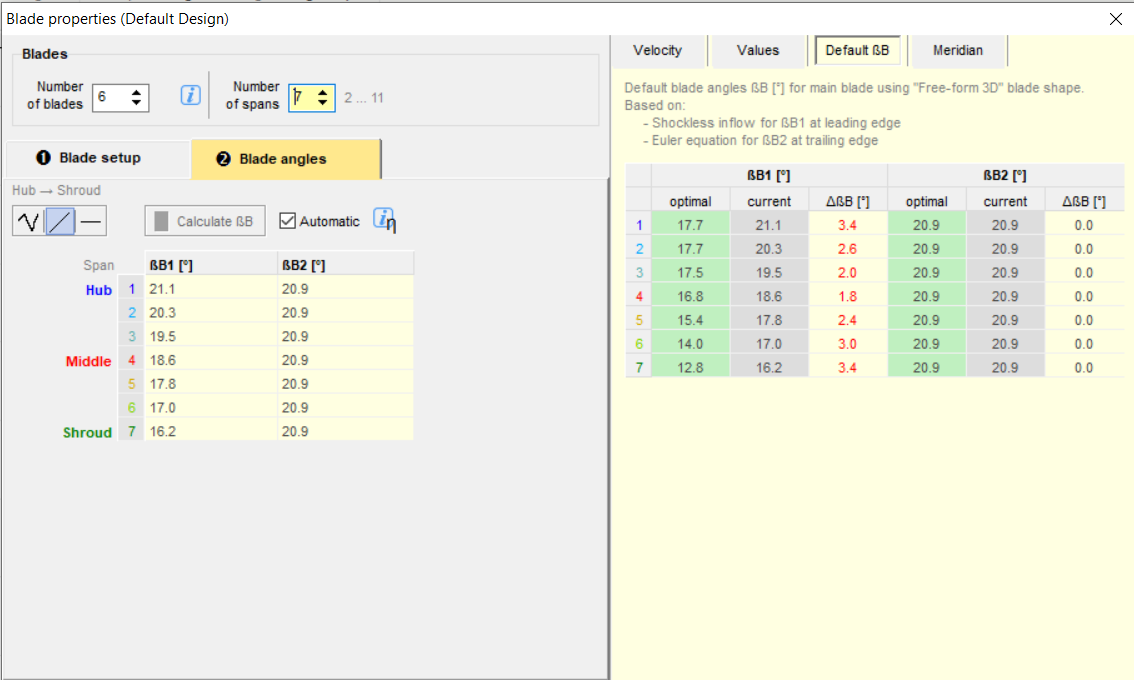
\includegraphics[width=0.94\linewidth,height=0.33\textheight,keepaspectratio]{figures/rId45.png}

\caption{Blade angles calculated automatically by CFturbo.}\end{figure}

Next, design the mean lines. The source cites a reference-book recommendation for a wrap angle of $100^\circ$--$130^\circ$, where wrap is the angle between the radial lines to the leading and trailing edges. A wrap angle of $115^\circ$ is chosen.

\begin{figure}[H]\centering

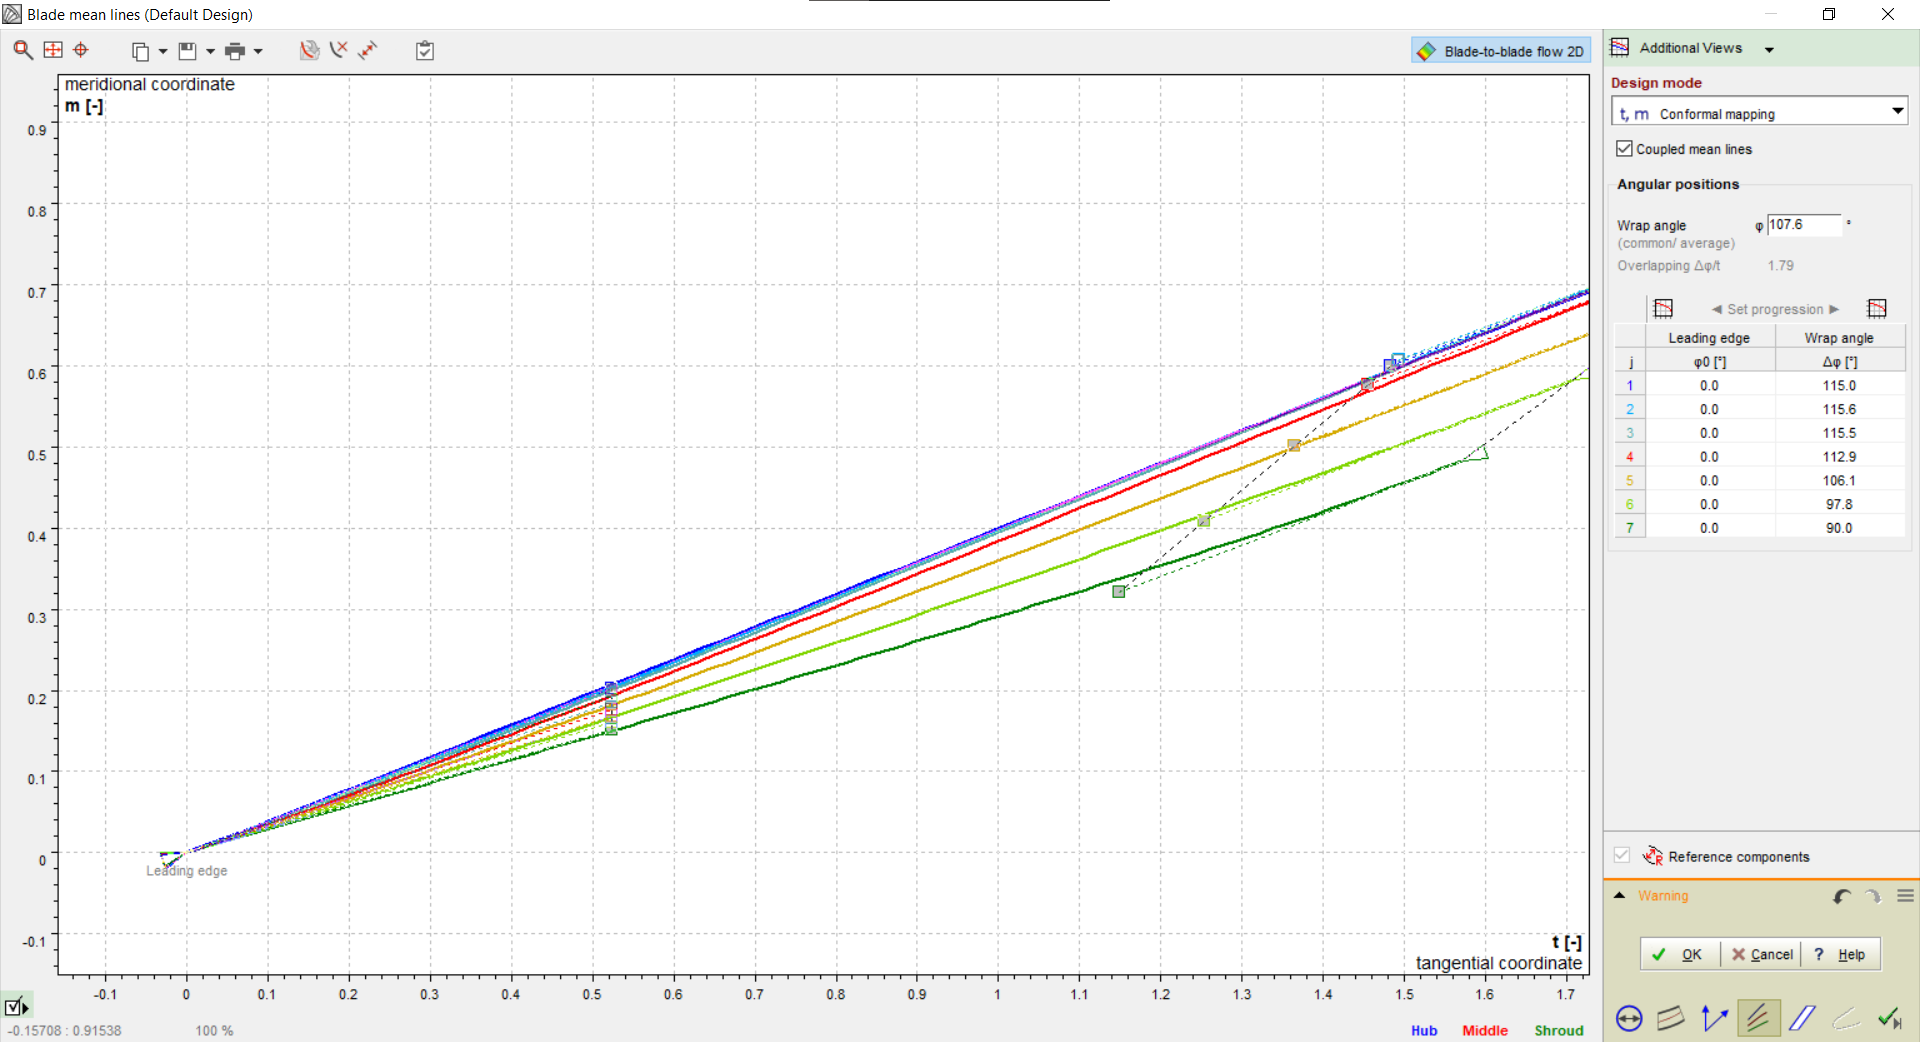
\includegraphics[width=0.94\linewidth,height=0.33\textheight,keepaspectratio]{figures/rId46.png}

\caption{Mean line design with the selected wrap angle.}\end{figure}

The blade-to-blade view is shown below. The visible continuation of the blade is attributed to the use of Free-form 3D geometry.

\begin{figure}[H]\centering

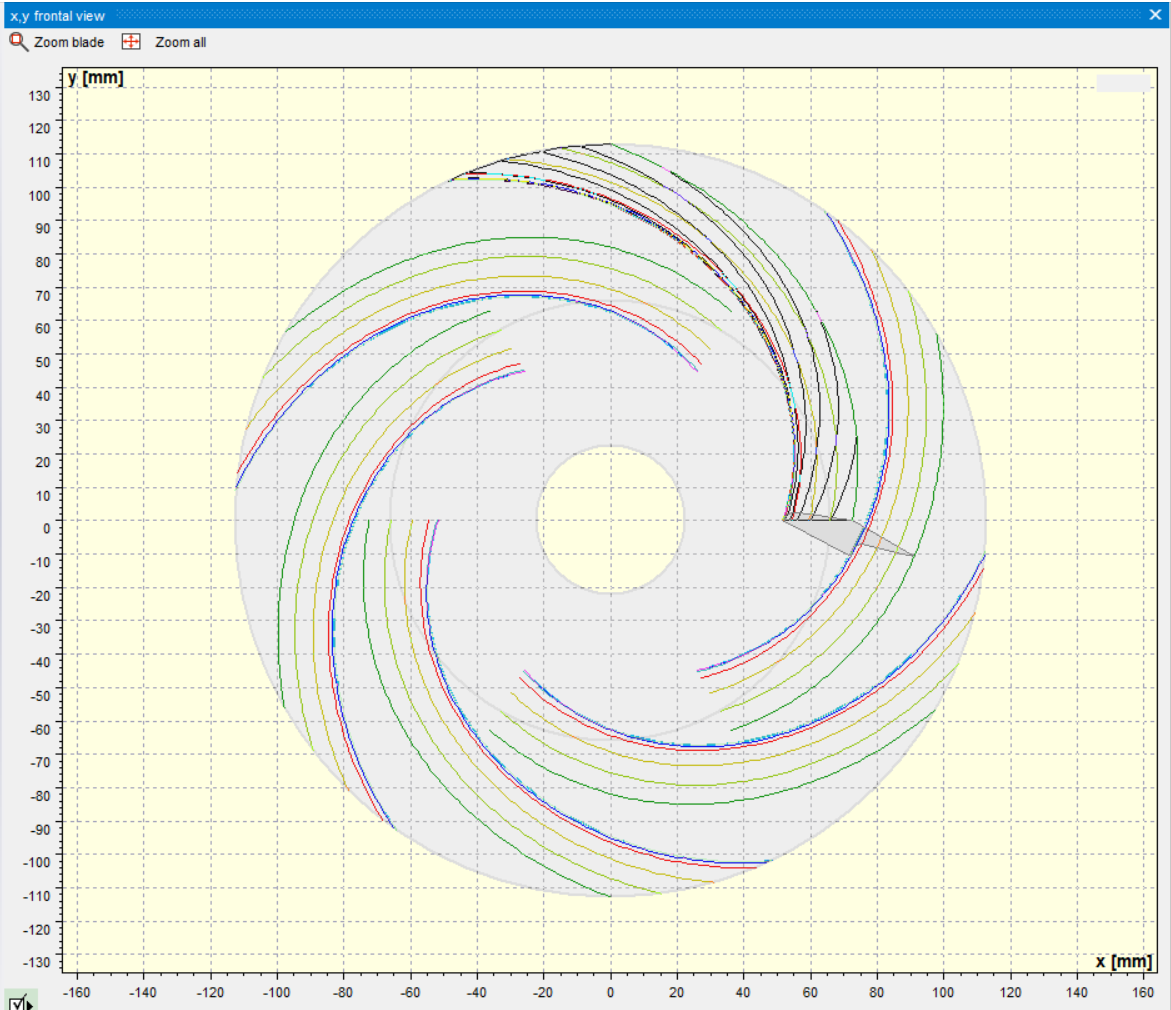
\includegraphics[width=0.94\linewidth,height=0.33\textheight,keepaspectratio]{figures/rId47.png}

\caption{Blade-to-blade view of the free-form geometry.}\end{figure}

The plot below shows blade angle along the mean line. The designer should avoid abrupt changes in the angle curves because they can promote flow separation and reduce hydraulic performance.

\begin{figure}[H]\centering

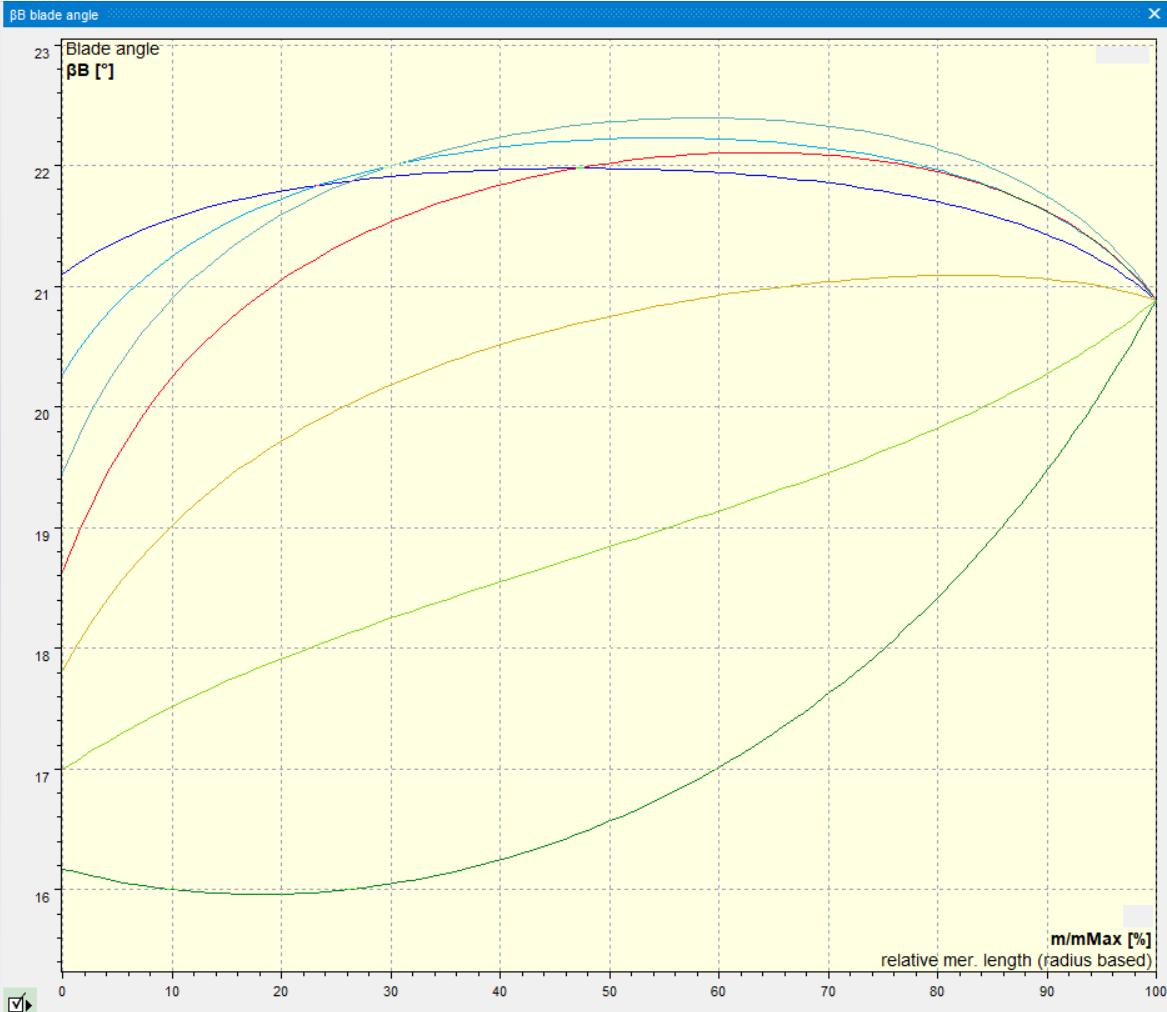
\includegraphics[width=0.94\linewidth,height=0.33\textheight,keepaspectratio]{figures/rId48.png}

\caption{Blade angle distributions along the mean lines.}\end{figure}

\subsection{Leading and trailing edge design}

Blade-edge location directly affects hydraulic behavior. The leading edge is placed in the impeller eye region, and the trailing edge at the outer diameter $D_2$. The source describes inclined edge geometry as a way to reduce stress concentration and provide smoother fluid entry.

The source recommends rounded, blade-like edge profiles rather than blunt, flat edges, describing the latter as producing stagnation and reduced hydraulic performance. It also calls for similar edge shapes from hub to shroud. These qualitative design statements are retained from the original report.

\begin{figure}[H]\centering

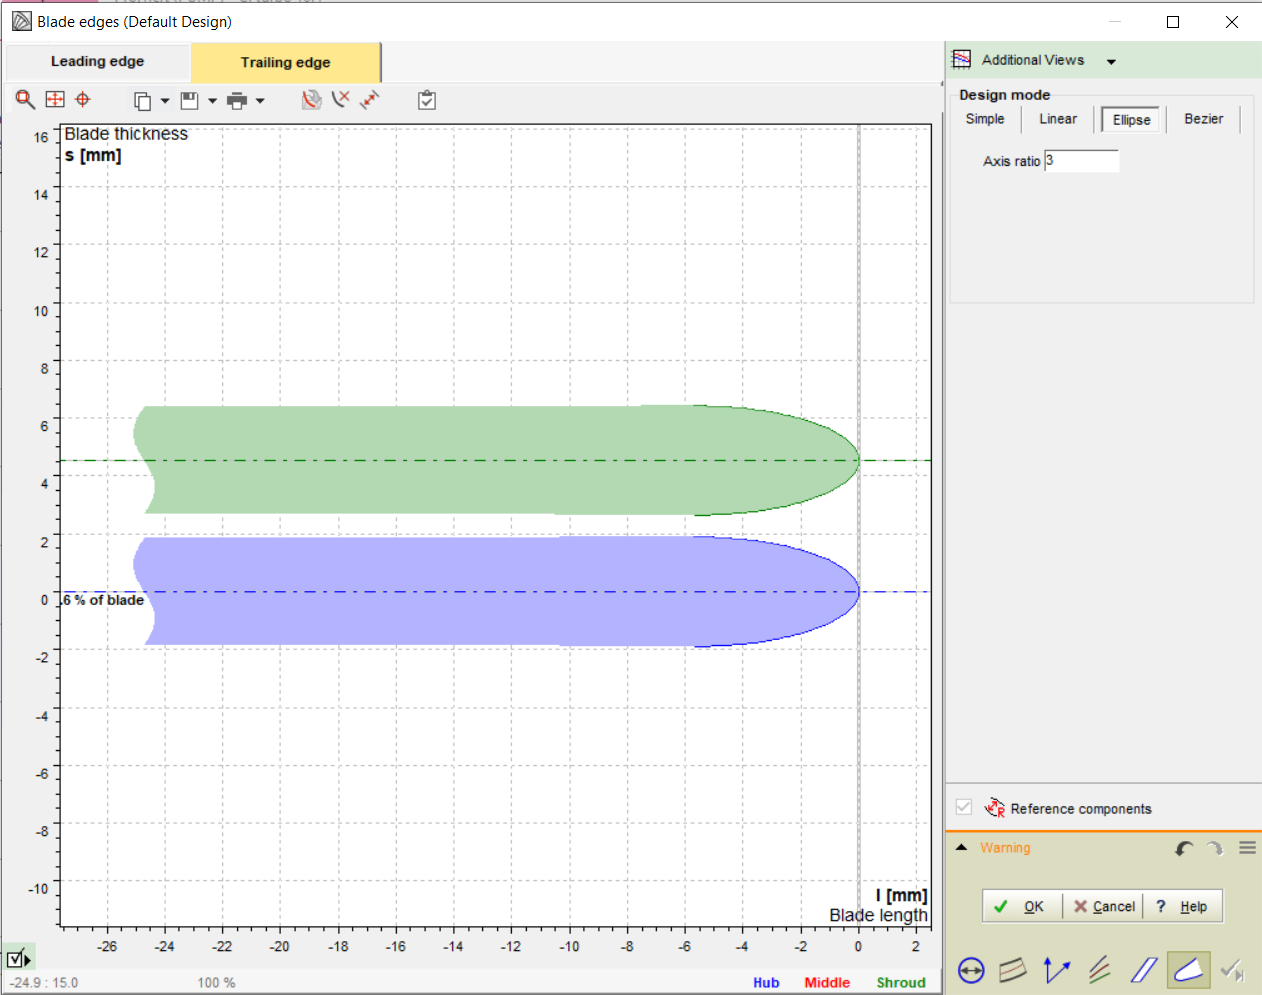
\includegraphics[width=0.94\linewidth,height=0.33\textheight,keepaspectratio]{figures/rId49.png}

\caption{Leading and trailing edge profile settings.}\end{figure}

\begin{figure}[H]\centering

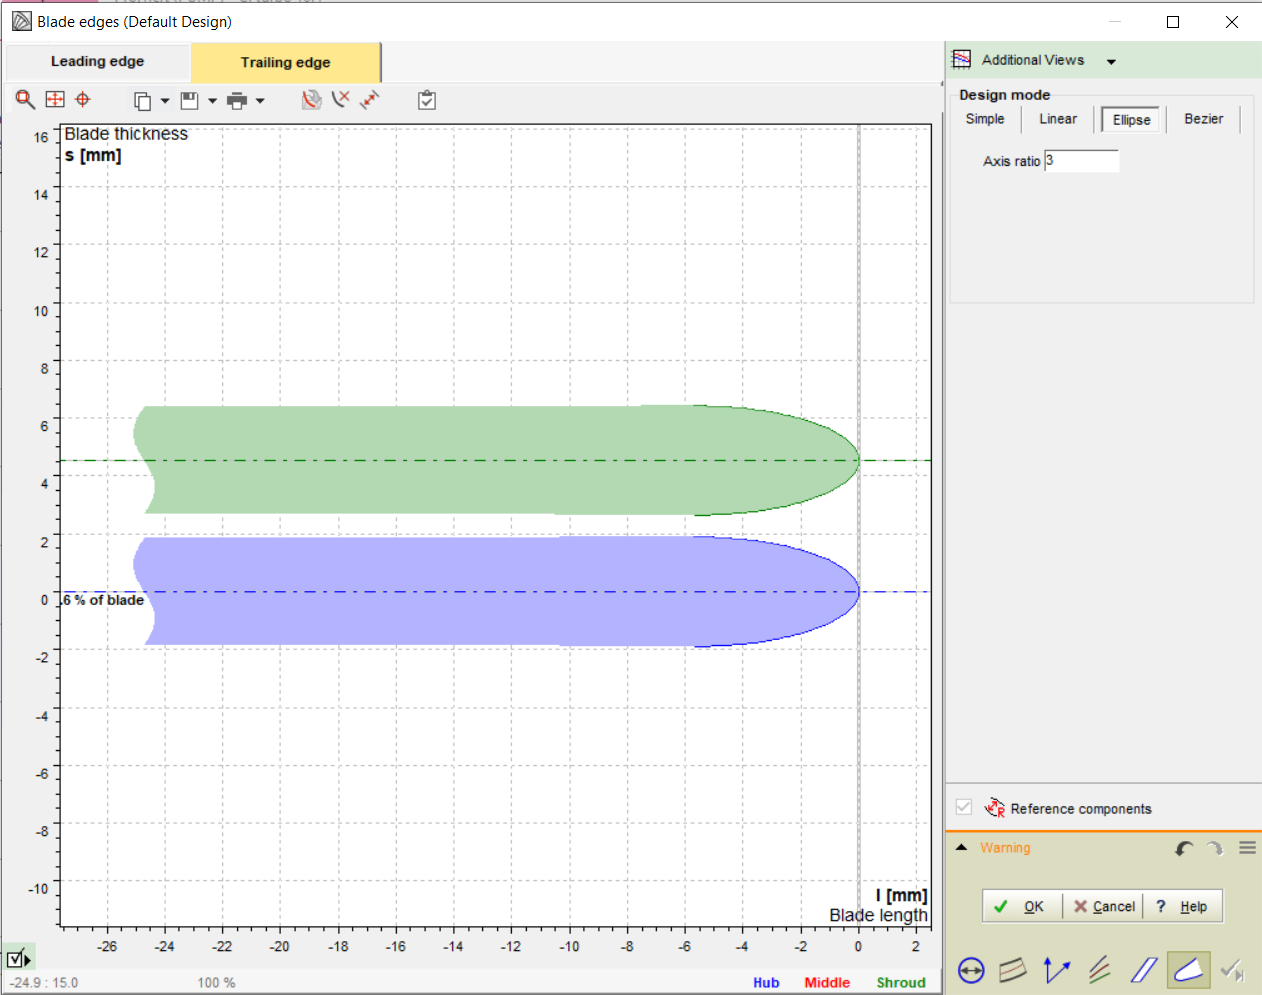
\includegraphics[width=0.94\linewidth,height=0.33\textheight,keepaspectratio]{figures/rId49.png}

\caption{Repeated edge-design view retained from the original report.}\end{figure}

The same blade-like profile can also be observed in the front view.

\begin{figure}[H]\centering

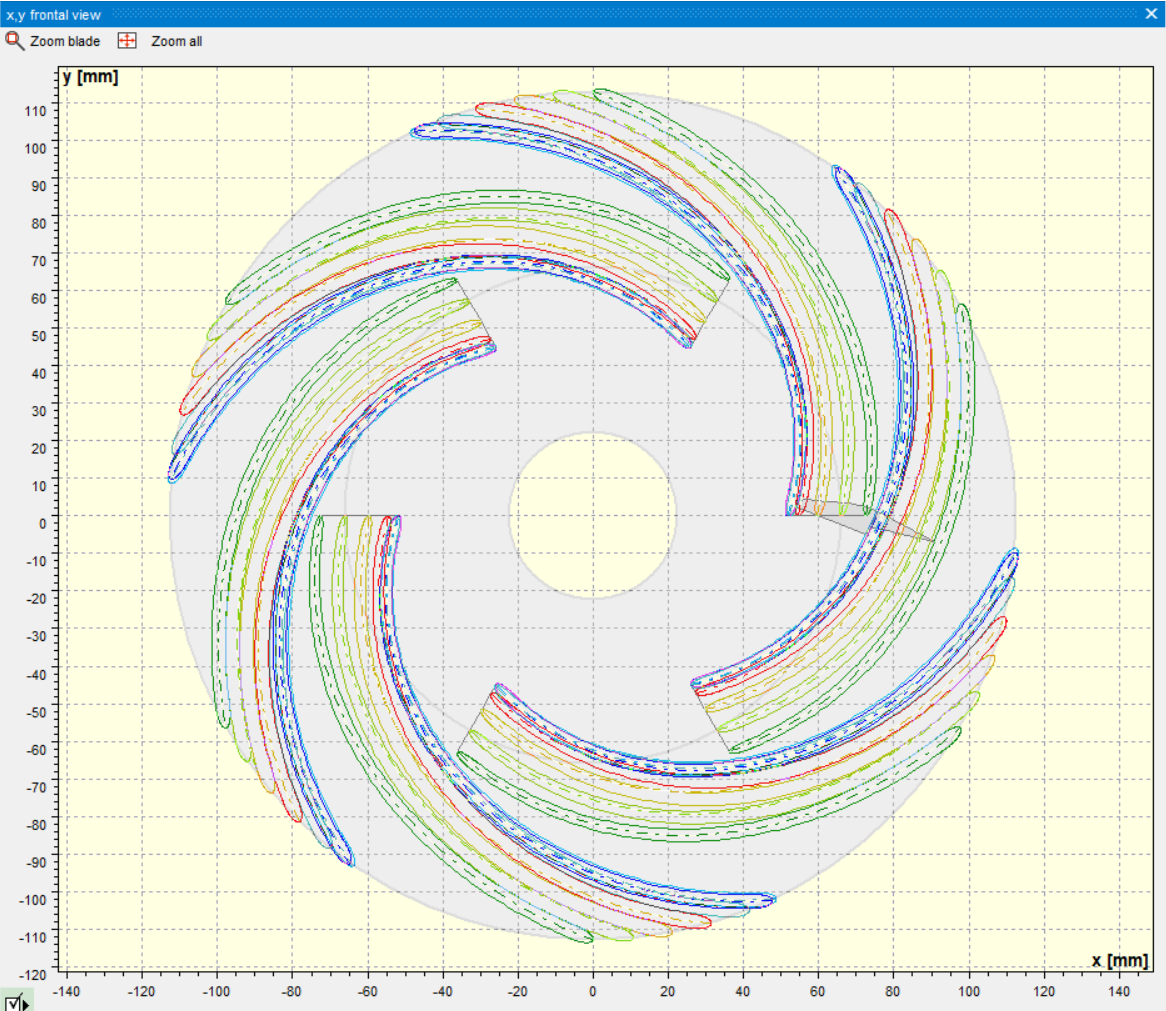
\includegraphics[width=0.94\linewidth,height=0.33\textheight,keepaspectratio]{figures/rId50.png}

\caption{Front view of the blade edge geometry.}\end{figure}

\subsection{Preliminary assessment in CFturbo}

The source presents the CFturbo stage as an initial performance assessment and geometric-design check before more detailed CFD analysis.

The final three-dimensional impeller geometry can now be viewed.

\begin{figure}[H]\centering

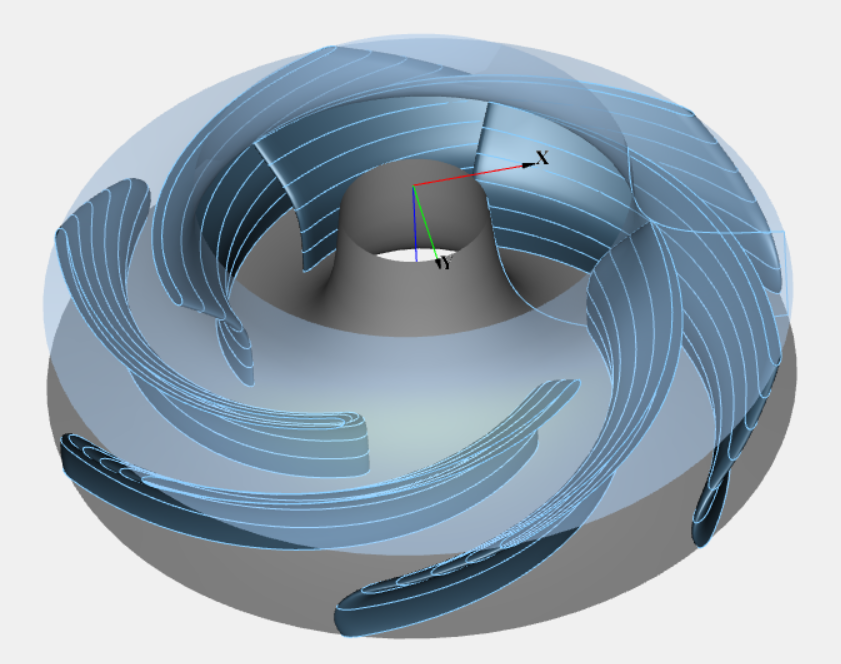
\includegraphics[width=0.94\linewidth,height=0.33\textheight,keepaspectratio]{figures/rId51.png}

\caption{Three-dimensional view of the impeller design.}\end{figure}

\begin{figure}[H]\centering

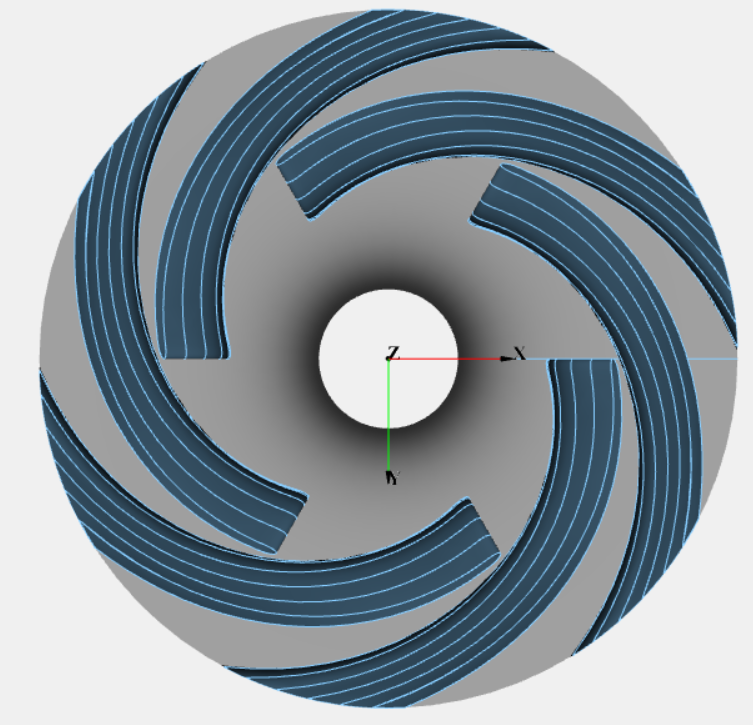
\includegraphics[width=0.94\linewidth,height=0.33\textheight,keepaspectratio]{figures/rId52.png}

\caption{Top view of the impeller geometry.}\end{figure}

\begin{figure}[H]\centering

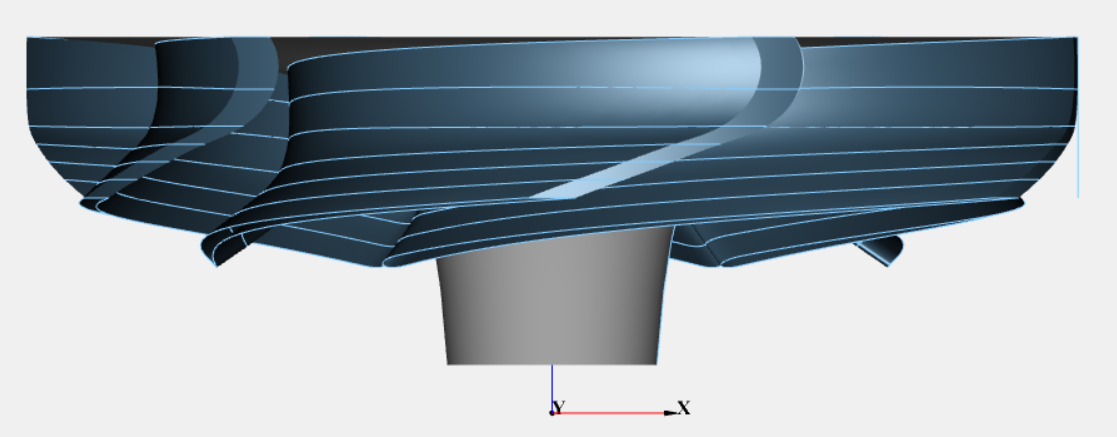
\includegraphics[width=0.94\linewidth,height=0.33\textheight,keepaspectratio]{figures/rId53.png}

\caption{Side detail of the impeller geometry.}\end{figure}

\begin{figure}[H]\centering

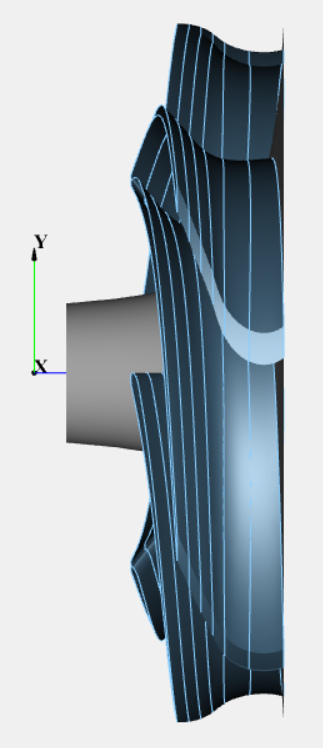
\includegraphics[width=0.94\linewidth,height=0.33\textheight,keepaspectratio]{figures/rId54.png}

\caption{Axial side view of the impeller.}\end{figure}

\begin{figure}[H]\centering

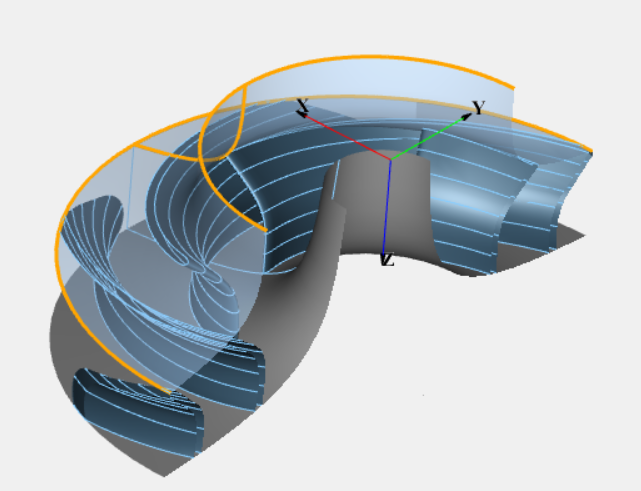
\includegraphics[width=0.94\linewidth,height=0.33\textheight,keepaspectratio]{figures/rId55.png}

\caption{Perspective detail showing the blade passage.}\end{figure}

Under Impeller, open Model Finishing and select Extend Blade Only.

\begin{figure}[H]\centering

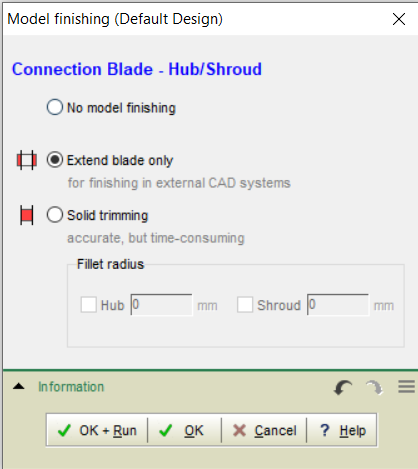
\includegraphics[width=0.94\linewidth,height=0.33\textheight,keepaspectratio]{figures/rId56.png}

\caption{Model finishing with Extend Blade Only selected.}\end{figure}

Export the model in STEP and SWB formats.

\subsection{Assessment objectives and workflow}

\textbf{Velocity and pressure assessment.} The source describes analytical and semi-empirical estimates of relative velocity and static pressure along the interblade passage, intended to help identify regions susceptible to abrupt pressure reduction.

\textbf{Cavitation assessment.} The source discusses examining low-pressure regions near the leading edge and estimating the required net positive suction head, NPSHr. For this pump, the design should be checked so that the local pressure does not fall below the vapor pressure of water. The figure below contains empirical NPSHr estimates; it does not establish a resolved cavitating-flow simulation.

\begin{figure}[H]\centering

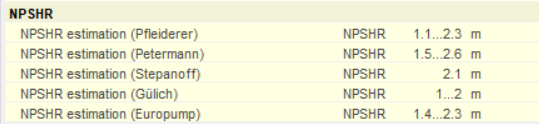
\includegraphics[width=0.94\linewidth,height=0.33\textheight,keepaspectratio]{figures/rId57.png}

\caption{Empirical NPSHr estimates displayed by CFturbo.}\end{figure}

\textbf{Blade loading.} The source proposes examining the pressure difference between the suction and pressure surfaces. A smooth loading distribution is described as desirable for limiting separation losses. An abrupt reduction in loading would motivate revising the blade-angle curves. No resolved blade-pressure dataset is supplied in the archive.

\textbf{Three-dimensional outputs and model transfer.} After reviewing the preliminary calculations, dimensions, and angles, the final impeller geometry is prepared for CAD export. Standard formats such as STEP or IGES can transfer geometry to fluid-analysis environments such as ANSYS CFX or Fluent, or to CAD systems such as SolidWorks. The supplied archive contains STEP and SWB exports; IGES and downstream CFD cases are not included.

\begin{figure}[H]\centering

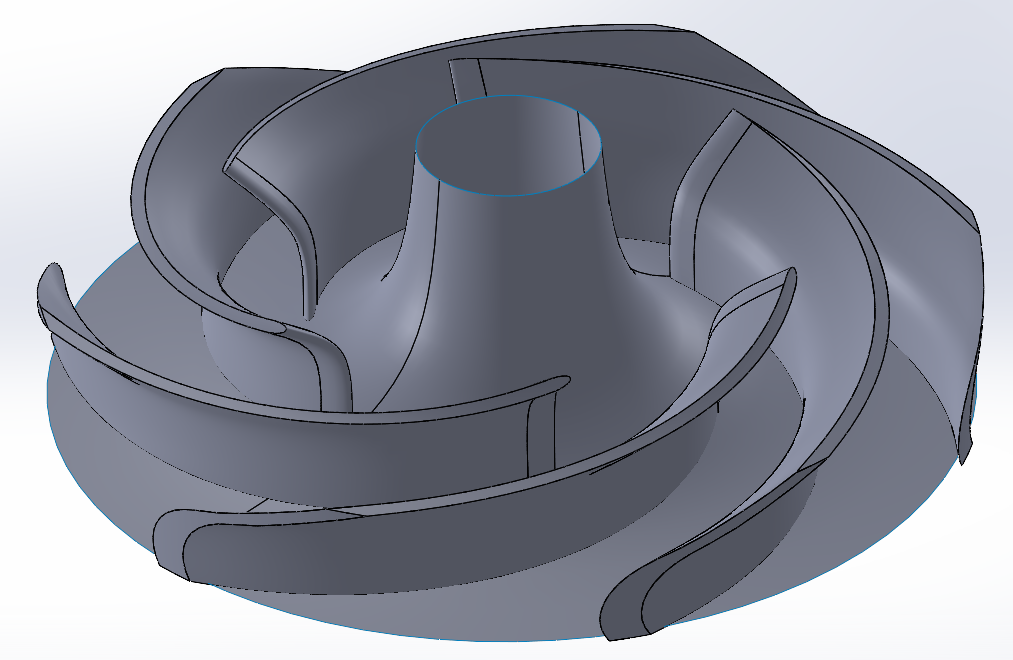
\includegraphics[width=0.48\linewidth,height=0.38\textheight,keepaspectratio]{figures/rId58.png}\hfill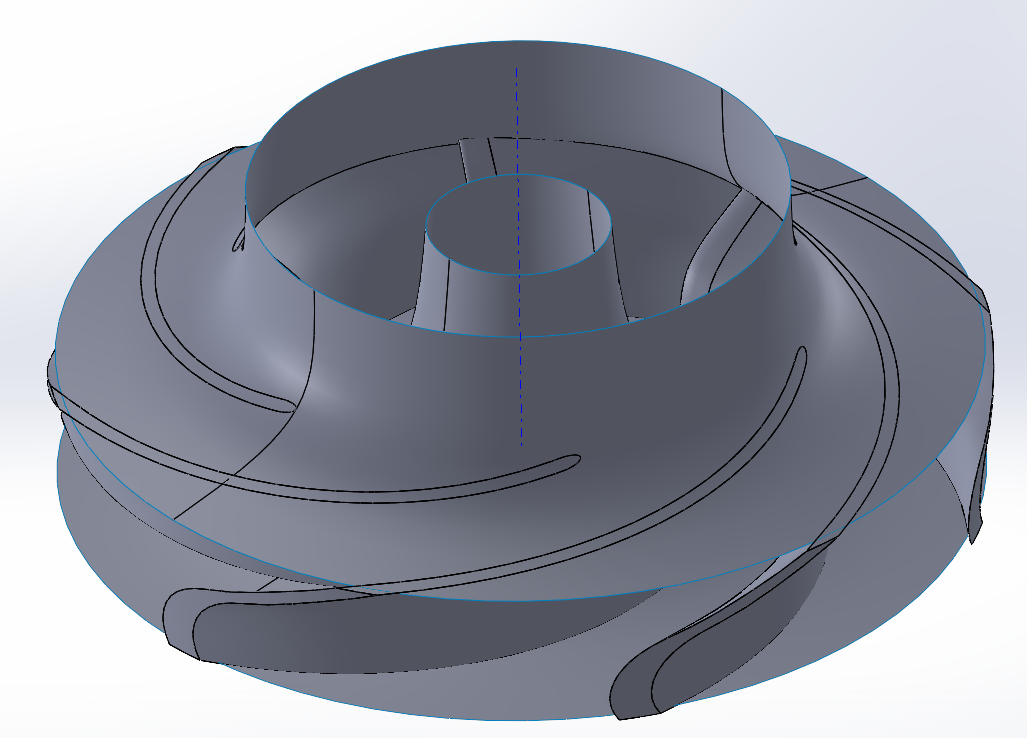
\includegraphics[width=0.48\linewidth,height=0.38\textheight,keepaspectratio]{figures/rId59.png}

\caption{CAD views of the impeller after geometry transfer.}\end{figure}

The source concludes that the final CFturbo model agrees reasonably with the Phase One calculations and offers a basis for physical manufacture or more detailed numerical testing. This conclusion is retained as the authors' assessment; the saved-model differences and the absence of independent validation are documented in the editorial appendix.

\FloatBarrier\clearpage\appendix
\section{Editorial Review and Saved Model Comparison}
This appendix was added during English preparation. It distinguishes the source report from values inspected in the supplied files. The CFturbo and SolidWorks projects have not been opened or recomputed in their native applications.

\subsection{Project scope and validation status}
The archive contains one Persian report, a CFturbo design file, a STEP export, a SolidWorks macro, two main SolidWorks parts, and two further parts in a folder named \texttt{Junk}. No CFD solver project, mesh, flow-field dataset, or experimental test results were supplied. Empirical NPSHr estimates and geometric diagnostic curves do not demonstrate a cavitation simulation or validate pump performance. The quoted 84.5\% catalog efficiency is a source datum, while the 90\% hydraulic efficiency is a design assumption; neither is a measured efficiency of the new impeller.

The source identifies the pump as both 200-100 and 100-200. The repository uses the descriptive project name instead of asserting that these are distinct pump models. The full Pumpiran catalog and the unspecified course reference book were not supplied as standalone references.

\subsection{Hand calculations and terminology}
The source's single arc formula gives approximately 121.11 mm when evaluated using $R_1=62.5$ mm, $R_2=104.5$ mm, $\beta'_1=25^\circ$, and $\beta'_2=35^\circ$, rather than the stated 120.9 mm. This small discrepancy should be reconciled with the exact sketch dimensions before manufacturing use.

The expression $\sqrt{(R_1^2+R_2^2)/2}=86.1002$ mm is the root mean square of the radii, not their geometric mean. The geometric mean would be $\sqrt{R_1R_2}=80.8161$ mm. The source's expression and reported 86.1 mm are retained in the translated body.

Using the same arc-radius formula with the stated intermediate radius and angles gives about 97.85 mm and 158.88 mm, close to the reported 97.7 mm and 159.1 mm. The later tangent-based drawing uses a different continuation construction and a radius of 568.39 mm. These are different constructions in the source; the report does not establish their equivalence.

For that final continuation, the angle associated with $R_F$ is $\beta'_F=5.26^\circ$. The explanatory source sentence calls it $\beta'_2$, although $\beta'_2=35^\circ$ is the separate outlet angle. The displayed equation and the reported 568.39 mm use the intended $\beta'_F$ notation.

The specific speed near 38.36 uses $N$ in rpm, $Q$ in $\mathrm{m^3/s}$, and $H$ in meters. This is the conventional European-style specific-speed value often denoted $n_q$; numerical specific-speed values depend on the unit convention and should not be compared across conventions without conversion.

\subsection{Suction connection and shaft diameter}
DN 125 describes the nominal suction connection shown in the catalog drawing; it is not a shaft diameter. The source separately gives a 32 mm coupling-shaft diameter and a 45 mm hub diameter. In the CFturbo main-dimensions interface, the suction-diameter field and the shaft sizing section are separate. The source's narrative confuses them during the standard-diameter selection step.

A catalog flange designation also does not by itself require the internal impeller eye diameter to be exactly 125 mm. That value is an assumption in the preliminary hand design. A point within the displayed Cordier recommendation region is a design heuristic, not independent hydraulic or mechanical validation.

\subsection{Parameters stored in the native CFturbo project}
The project XML records CFturbo version \texttt{10.4.5.27}, with format version \texttt{10.4}. Its global setup stores a rotational frequency of $24.1667\ \mathrm{s^{-1}}$ (1450 rpm), a mass flow of $34.7222\ \mathrm{kg/s}$, density $1000\ \mathrm{kg/m^3}$, and specific energy $132.435\ \mathrm{J/kg}$. These correspond to $125\ \mathrm{m^3/h}$ and a head of 13.5 m using $g=9.81\ \mathrm{m/s^2}$.

The following are stored parameter values, not independently regenerated geometry measurements:
\begin{table}[H]\centering\small
\caption{Preliminary design versus the supplied saved CFturbo state.}
\begin{tabular}{p{0.34\linewidth}p{0.24\linewidth}p{0.32\linewidth}}\toprule
Quantity & Preliminary report & Saved project\\\midrule
Outlet diameter & 209 mm & 225.8 mm\\
Outlet width & 32 mm & 34.55 mm\\
Eye or suction diameter & Eye assumed 125 mm & Suction field 132.5 mm\\
Hub diameter & 45 mm & 45 mm\\
Blade count & 6 & 6\\
Span count & 7 in CFturbo stage & 7\\
Blade form & Free-form 3D selected & FreeForm\\
Shroud and splitters & Shrouded, no splitters & Same settings\\
Hydraulic efficiency & 0.90 assumption & Global EtaC 0.90; component EtaH 0.912\\\bottomrule
\end{tabular}\end{table}
The saved component stores inlet-angle entries of approximately $21.10^\circ$ and $16.17^\circ$, and outlet-angle entries of approximately $20.89^\circ$ at both listed endpoints. The preliminary $25^\circ$ and $35^\circ$ angles therefore do not describe the final saved blade-angle values. This is consistent with the narrative later allowing automatic angle calculation, but the stages must not be presented as identical.

Similarly, the saved thickness arrays contain 3.2 mm entries for \texttt{s1} and 3.8 mm entries for \texttt{s2}, which differ from the prose's proposed hub and shroud values. Their exact leading/trailing and span assignments should be confirmed in CFturbo before claiming a particular final thickness distribution. The native file also stores some empirical coefficients independently of the resulting manually adjusted dimensions; a saved coefficient should not be assumed to equal a ratio recomputed from all final dimensions.

\subsection{CAD deliverables and reproducibility}
The STEP export contains solid-body, surface, and curve entities. It should not be described as one verified watertight manufacturing solid merely because the filename ends in \texttt{.stp}. The native SolidWorks part files have not been inspected in SolidWorks, so their association with a particular blade construction is not inferred from generic names such as \texttt{Part1} and \texttt{Part2}.

The \texttt{.swb} file is an ASCII SolidWorks macro generated by CFturbo 10.4.5, with a \texttt{main} entry point. It creates geometric features and requires SolidWorks; it is not a standalone numerical simulation program. Original CAD bytes are retained in the repository package, including the separately labeled archive parts in \texttt{Solidworks/Junk}.

To reproduce the final design, open a copy of the native project in a compatible CFturbo installation, record its settings, and compare its geometry with the existing exports before saving. CFturbo's documented automatic calculations can alter values when old projects are opened in newer software. The software version, unit conventions, and saved design stage should therefore be recorded with any new export. Validate downstream CAD import and topology before using the geometry for meshing or manufacture.

\subsection{Documentation consulted during editorial review}
The following official CFturbo pages were consulted to clarify terminology and workflow. They are editorial references, not a replacement for the original catalog or course references.
\begin{enumerate}
\item \href{https://manual.cfturbo.com/en/cfturbo.html}{CFturbo Turbomachinery Design Software}.
\item \href{https://manual.cfturbo.com/en/md_parameters_pumpvent.html}{Centrifugal and mixed-flow pump parameters}.
\item \href{https://manual.cfturbo.com/en/prefunits_nq.html}{Specific speed definitions and unit conventions}.
\item \href{https://manual.cfturbo.com/en/automatic_updates.html}{Automatic calculations and opening older projects}.
\item \href{https://manual.cfturbo.com/BLADERUNNER/index.html}{BLADERUNNER and downstream CFD simulation workflow}.
\end{enumerate}
\end{document}
